\documentclass[12pt]{article}
\usepackage{hyperref}
\usepackage[warn]{mathtext}
\usepackage[T2A]{fontenc}
\usepackage[utf8]{inputenc}
\usepackage[russian]{babel}
\usepackage{cite}
\usepackage{amsfonts}
\usepackage{lineno}
\usepackage{subfig}
\usepackage{graphicx}
\usepackage{xcolor}
\usepackage{bm}
\usepackage{graphicx}
\usepackage{amssymb}
\usepackage{hyperref}
\usepackage[left=2cm,right=2cm,top=2cm,bottom=2cm]{geometry}
\usepackage{indentfirst}
\DeclareSymbolFont{T2Aletters}{T2A}{cmr}{m}{it}

\DeclareGraphicsExtensions{.png,.jpg,.svg,.pdf}
\author{Карцев Вадим}
\title{Лабораторная работа 1.2

Исследование эффекта Комптона}

\begin{document}

  \maketitle

  \textbf{Цель работы:} % TODO Дописать цель работы

  \textbf{В работе используется:} % TODO Дописать оборудование

  \section{Аннотация}

  \section{Теоретическая справка}

  \newpage
  \section{Обработка результатов}

    С помощью сцинтилляционного счетчика проведем замеры спектра и выясним
    зависимость положения фотопика от угла, под которым мы исследуем спектр
    рассеянных $\gamma$-лучей.

    Длительность замера спектра для каждого угла выберем такой, чтобы фотопик был
    в полной мере различим на спектрограмме.

    По спектрограммам на стр. \pageref{add:spectres} определим расположения
    фотопиков для раличных углов рассеяния.
    Ниже приведена таблица с результатами измерений для всех углов $\theta$.
    Погрешность измерения угла будем считать как половину деления разметки
    измерительного стола $\sigma_{\theta} = 0,5^{\circ}$.
    Погрешность положения фотопика возьмем как половину ширины вершины фотопика.
    Значения погрешности положения также приведены в таблице ниже.\\

    \begin{tabular}{|c||c|c|c|c|c|c|c|c|c|c|c|c|c|}
      \hline
      $\theta$ & $0^{\circ}$ & $10^{\circ}$ & $20^{\circ}$ & $30^{\circ}$ & $40^{\circ}$ & $50^{\circ}$ & $60^{\circ}$ & $70^{\circ}$ & $80^{\circ}$ & $90^{\circ}$ & $100^{\circ}$ & $110^{\circ}$ & $120^{\circ}$ \\ \hline
      $N$ & $912$ & $868$ & $790$ & $751$ & $665$ & $594$ & $536$ & $463$ & $424$ & $385$ & $353$ & $319$ & $282$ \\ \hline
      $\sigma_N$ & $8$ & $7$ & $20$ & $6$ & $8$ & $5$ & $4$ & $6$ & $6$ & $3$ & $5$ & $2$ & $6$ \\
      \hline
    \end{tabular}\\

    Погрешность для $1/N$ и $1 - \cos\theta$ будут считаться по формулам

    $$
      \sigma_{1/N} = \frac{1}{N} \varepsilon_N = \frac{1}{N} \frac{\sigma_N}{N}
      = \frac{\sigma_N}{N^2}; \hspace{0.5cm}
      \sigma_{1 - \cos\theta} = \sin(\theta) \sigma_{\theta}.
    $$

    \begin{figure}[h!]
      \center{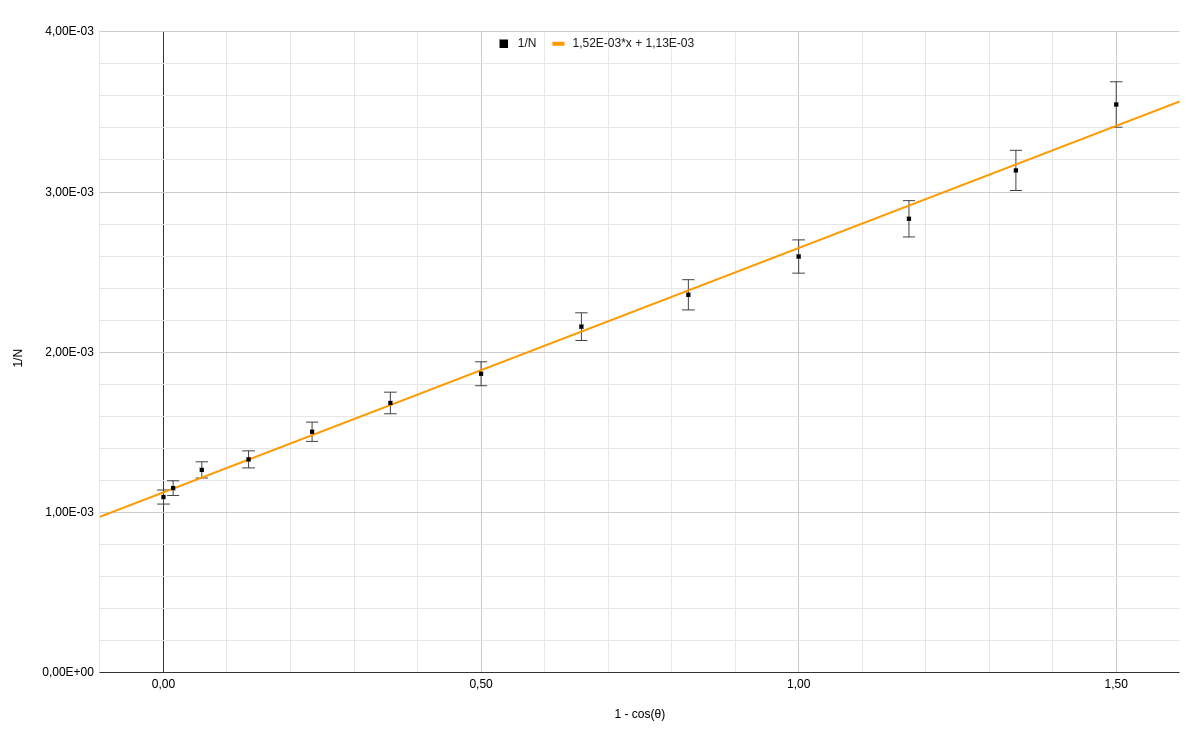
\includegraphics[width = \linewidth]{plot.png}}\\
      Рис 1. Зависимость
      \label{fig:oscillograme}
    \end{figure}

    По МНК получим коэффициент наклона и точку пересечения прямой с осью Y.
    Также вычислим погрешности для этих значений.

    $$
      A = \frac{\left<xy\right> - \left<x\right>\left<y\right>}{\left<x^2\right>
      - \left<x\right>^2}; \hspace{0.5cm} \sigma_A = \frac{1}{\sqrt{n}}
      \sqrt{\frac{\left<y^2\right> - \left<y\right>^2}{\left<x^2\right> -
      \left<x\right>^2} - A^2}
    $$

    $$
      \frac{1}{N(0)} = \left<y\right> - A \left<x\right>; \hspace{0.5cm}
      \sigma_{1/N(0)} = \sigma_A \sqrt{\left<x^2\right>}
    $$

    Из этих формул рассчитаем значения угла наклона и пересечения прямой с осью
    Y с погрешностями.

    $$
      N(0^{\circ}) = 888,28 \pm 17,57; \hspace{0.5cm}
      N(90^{\circ}) = 377,30 \pm 7,21
    $$

    Из вычисленных значений для $N(0^{\circ})$ и $N(90^{\circ})$ получим
    значение $mc^2$ и погрешность для него по следующим формулам

    $$
      mc^2 = E_{\gamma} \frac{N(90^{\circ})}{N(0^{\circ}) - N(90^{\circ})};
      \hspace{0.5cm}
      \sigma_{mc^2} = mc^2 \sqrt{\varepsilon_{N(0^{\circ})}^2 +
      \varepsilon_{N(90^{\circ})}^2}
    $$

    где

    $$
      \varepsilon_{N(0^{\circ})} = \frac{\sigma_{N(0^{\circ})}}{N(0^{\circ})};
      \hspace{0.5cm}
      \varepsilon_{N(90^{\circ})} = \frac{\sigma_{N(90^{\circ})}}{N(90^{\circ})}
    $$

    Таким образом получим результат $mc^2 = (488,51 \pm 13,43) кэВ$. Полученный
    результат имеет относительную погрешность $\varepsilon_{mc^2} = 2,75\%$.

  \section{Вывод}

  \newpage
  \section{Приложение}
  \label{add:spectres}

  \begin{figure}[h!]
    \begin{minipage}[h]{0.32\linewidth}
      \center{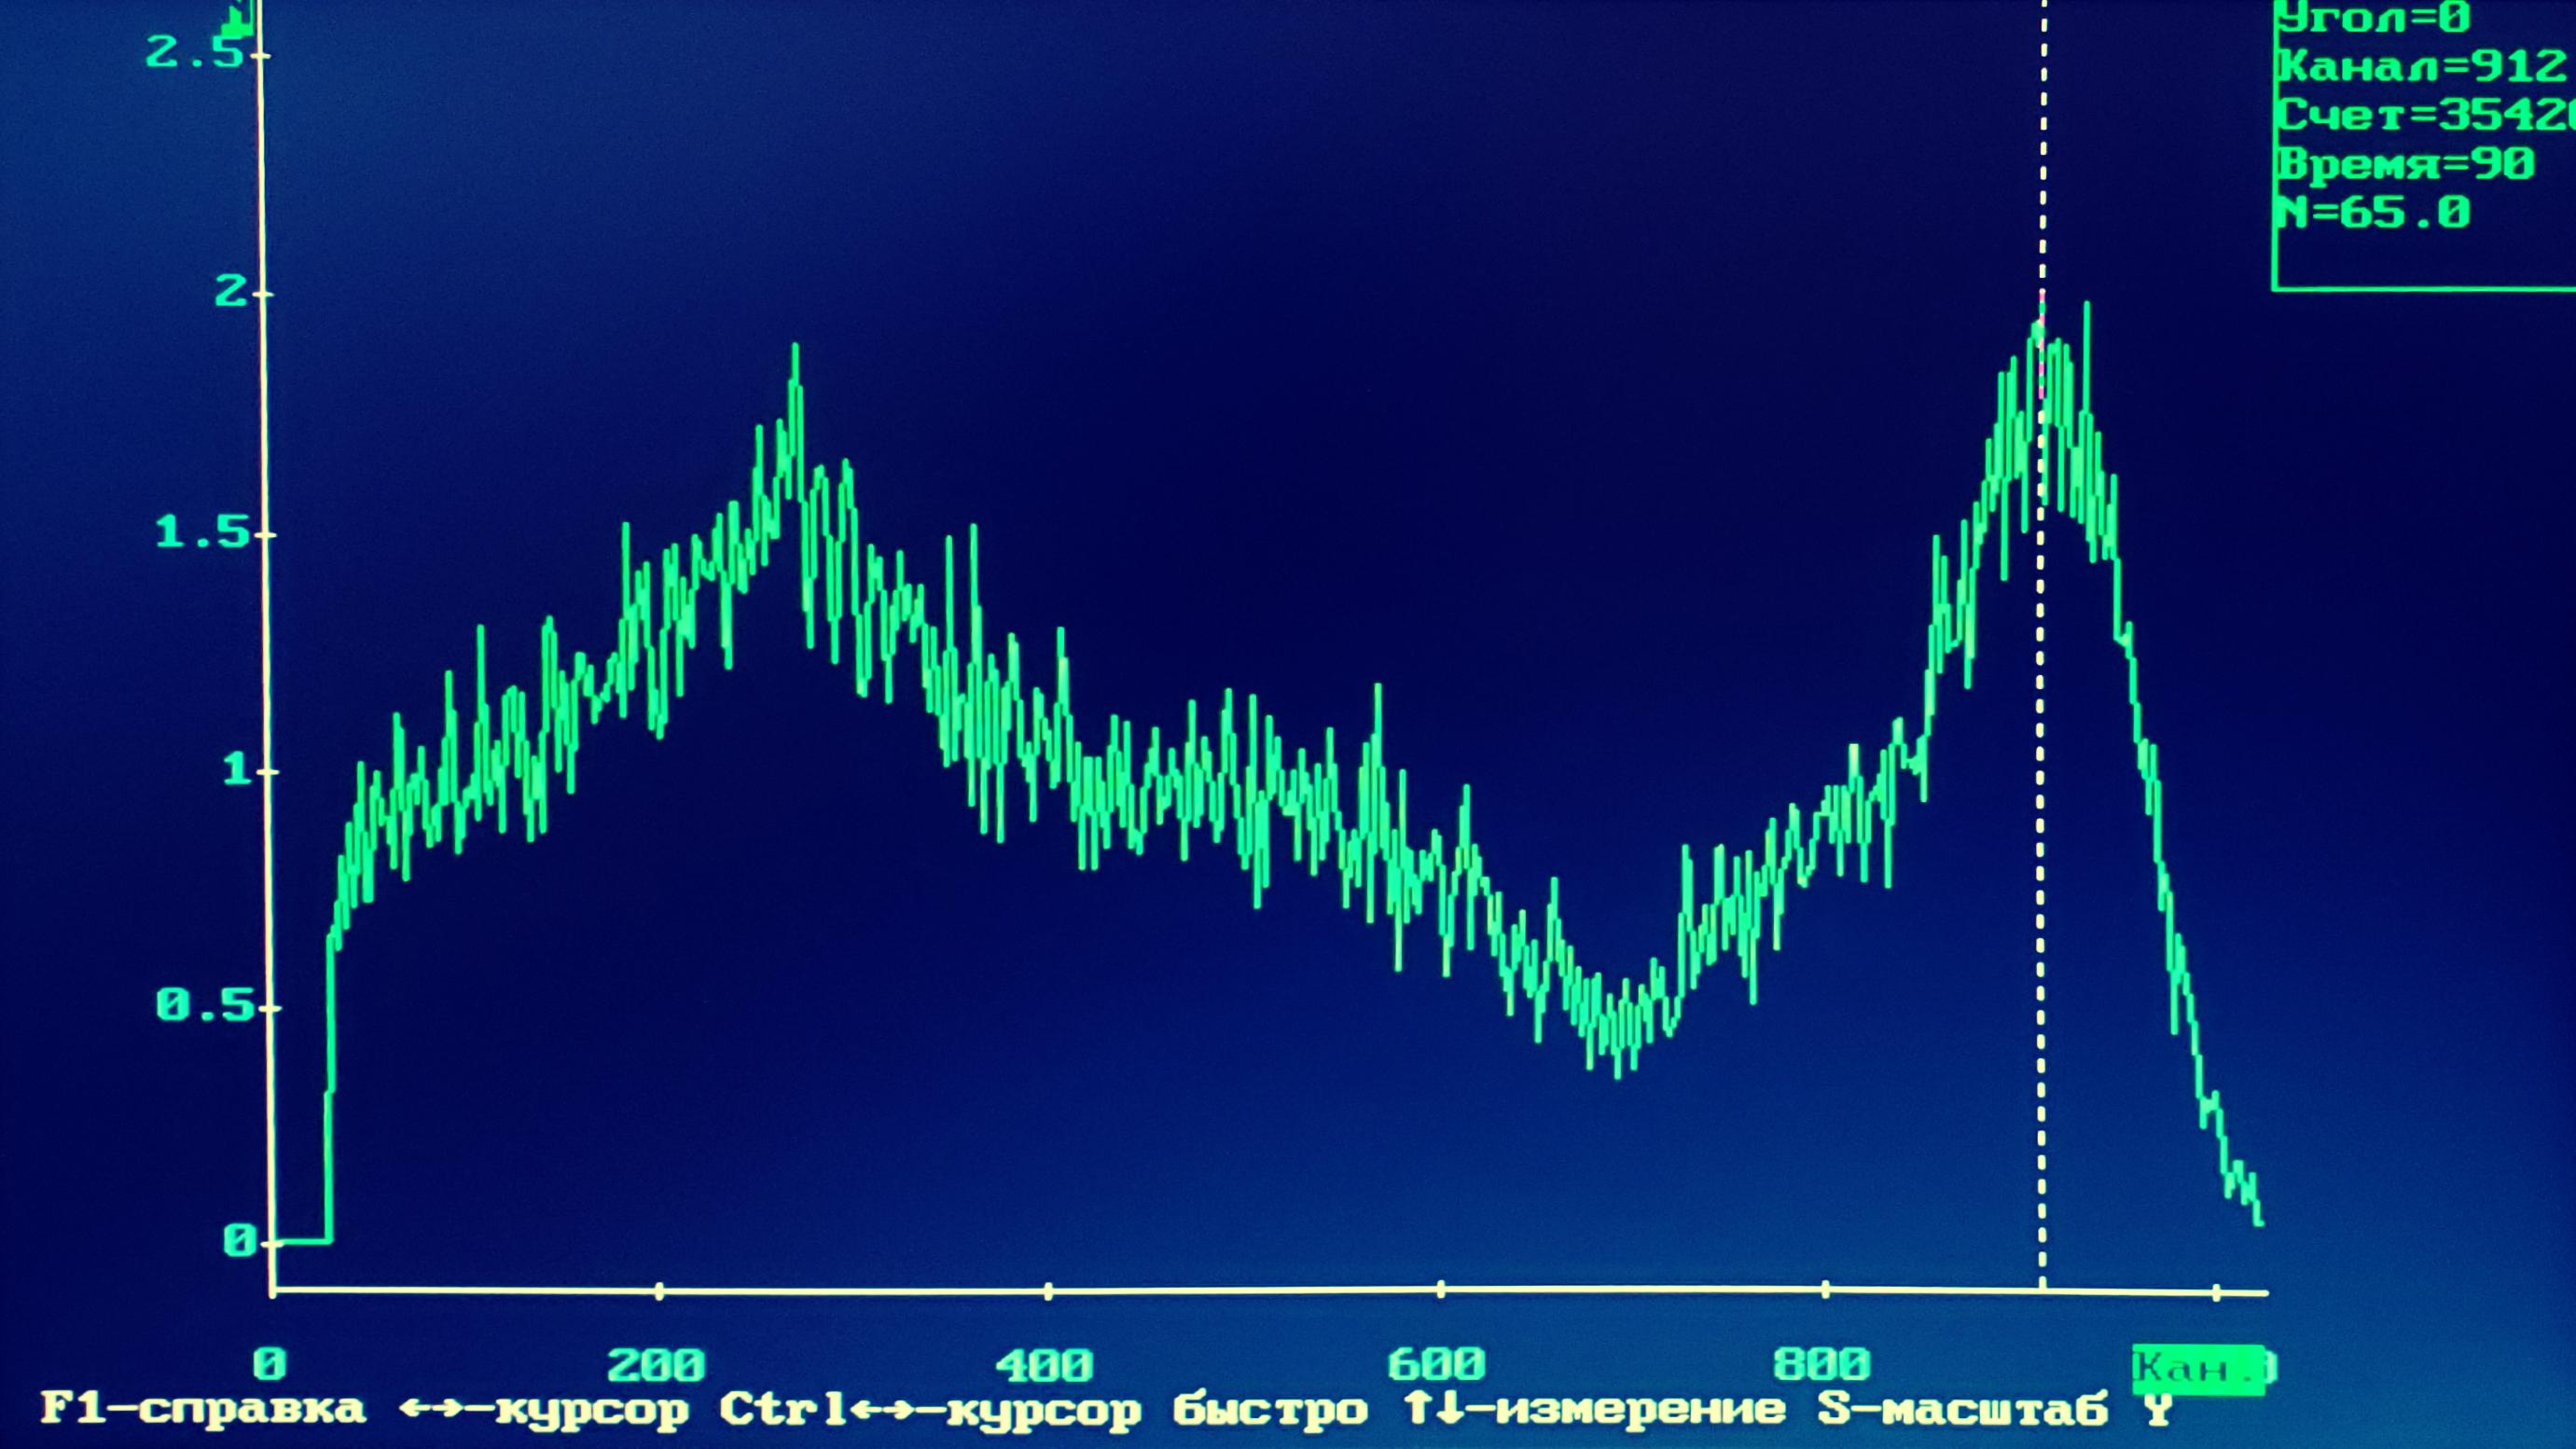
\includegraphics[width = \linewidth]{spectre0.jpg}}\\
      Рис 2. $\theta = 0^{\circ}$
    \end{minipage}
    \begin{minipage}[h]{0.32\linewidth}
      \center{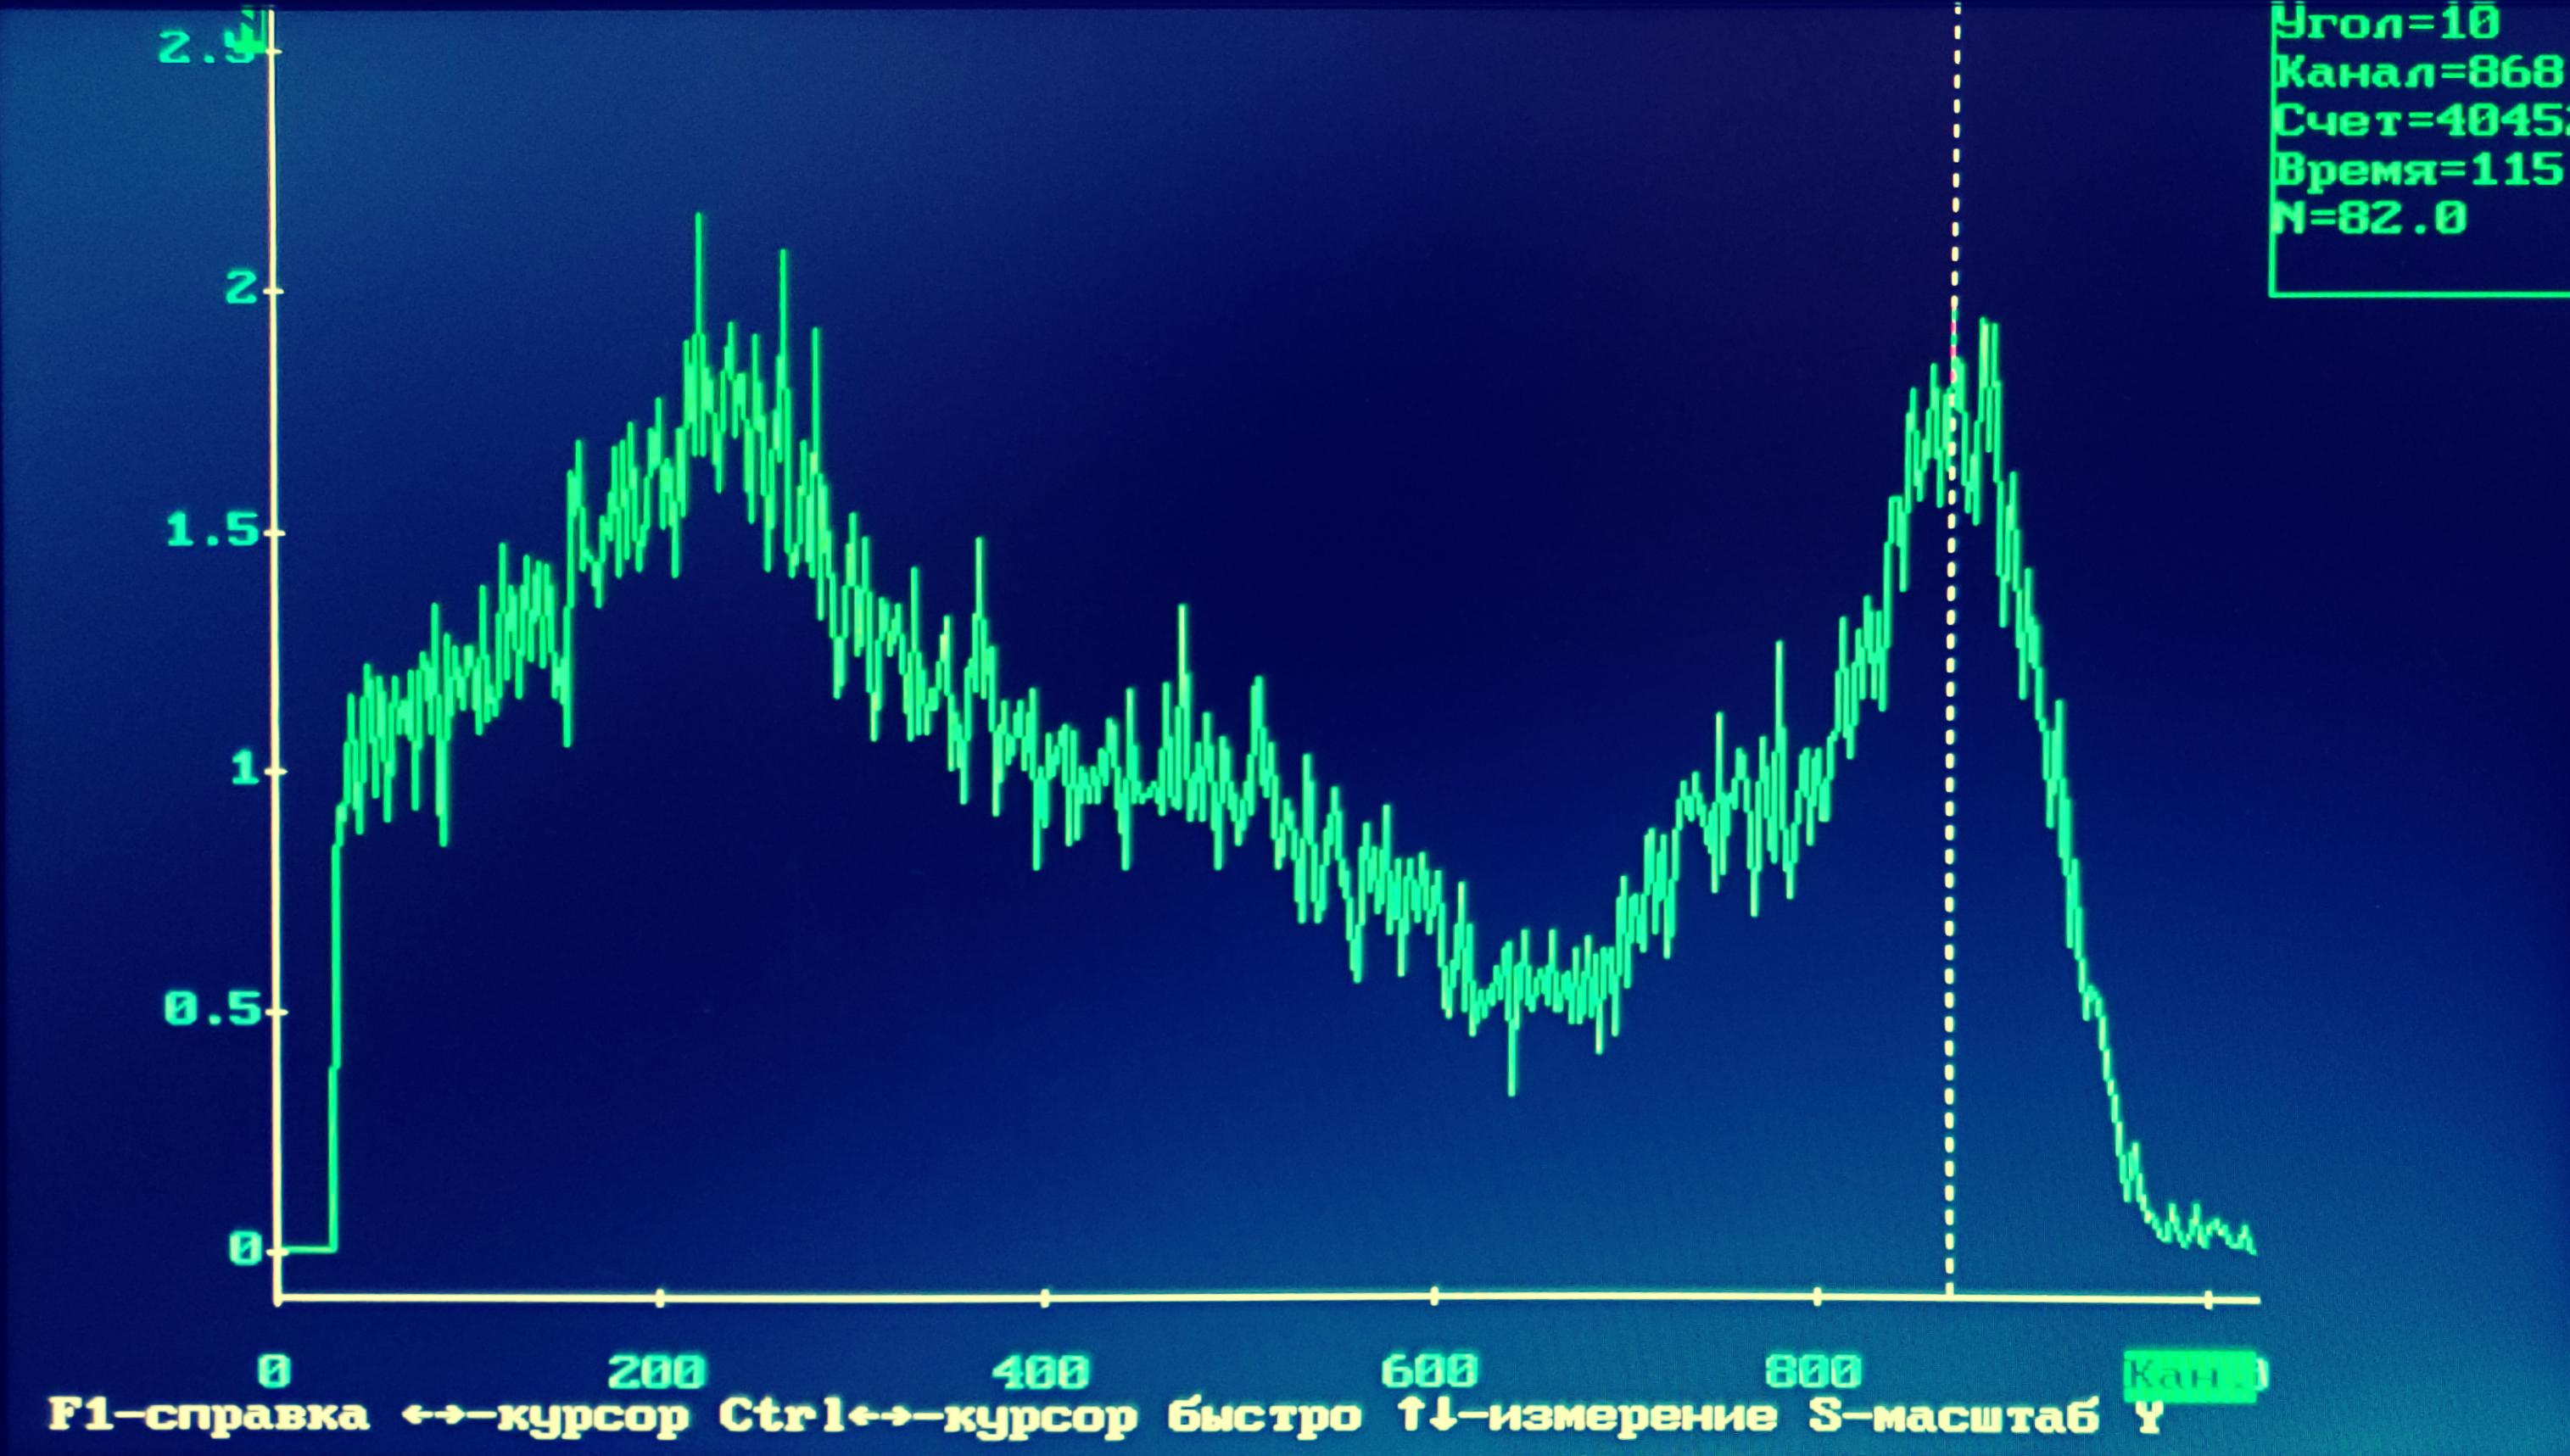
\includegraphics[width = \linewidth]{spectre10.jpg}}\\
      Рис 3. $\theta = 10^{\circ}$
    \end{minipage}
    \begin{minipage}[h]{0.32\linewidth}
      \center{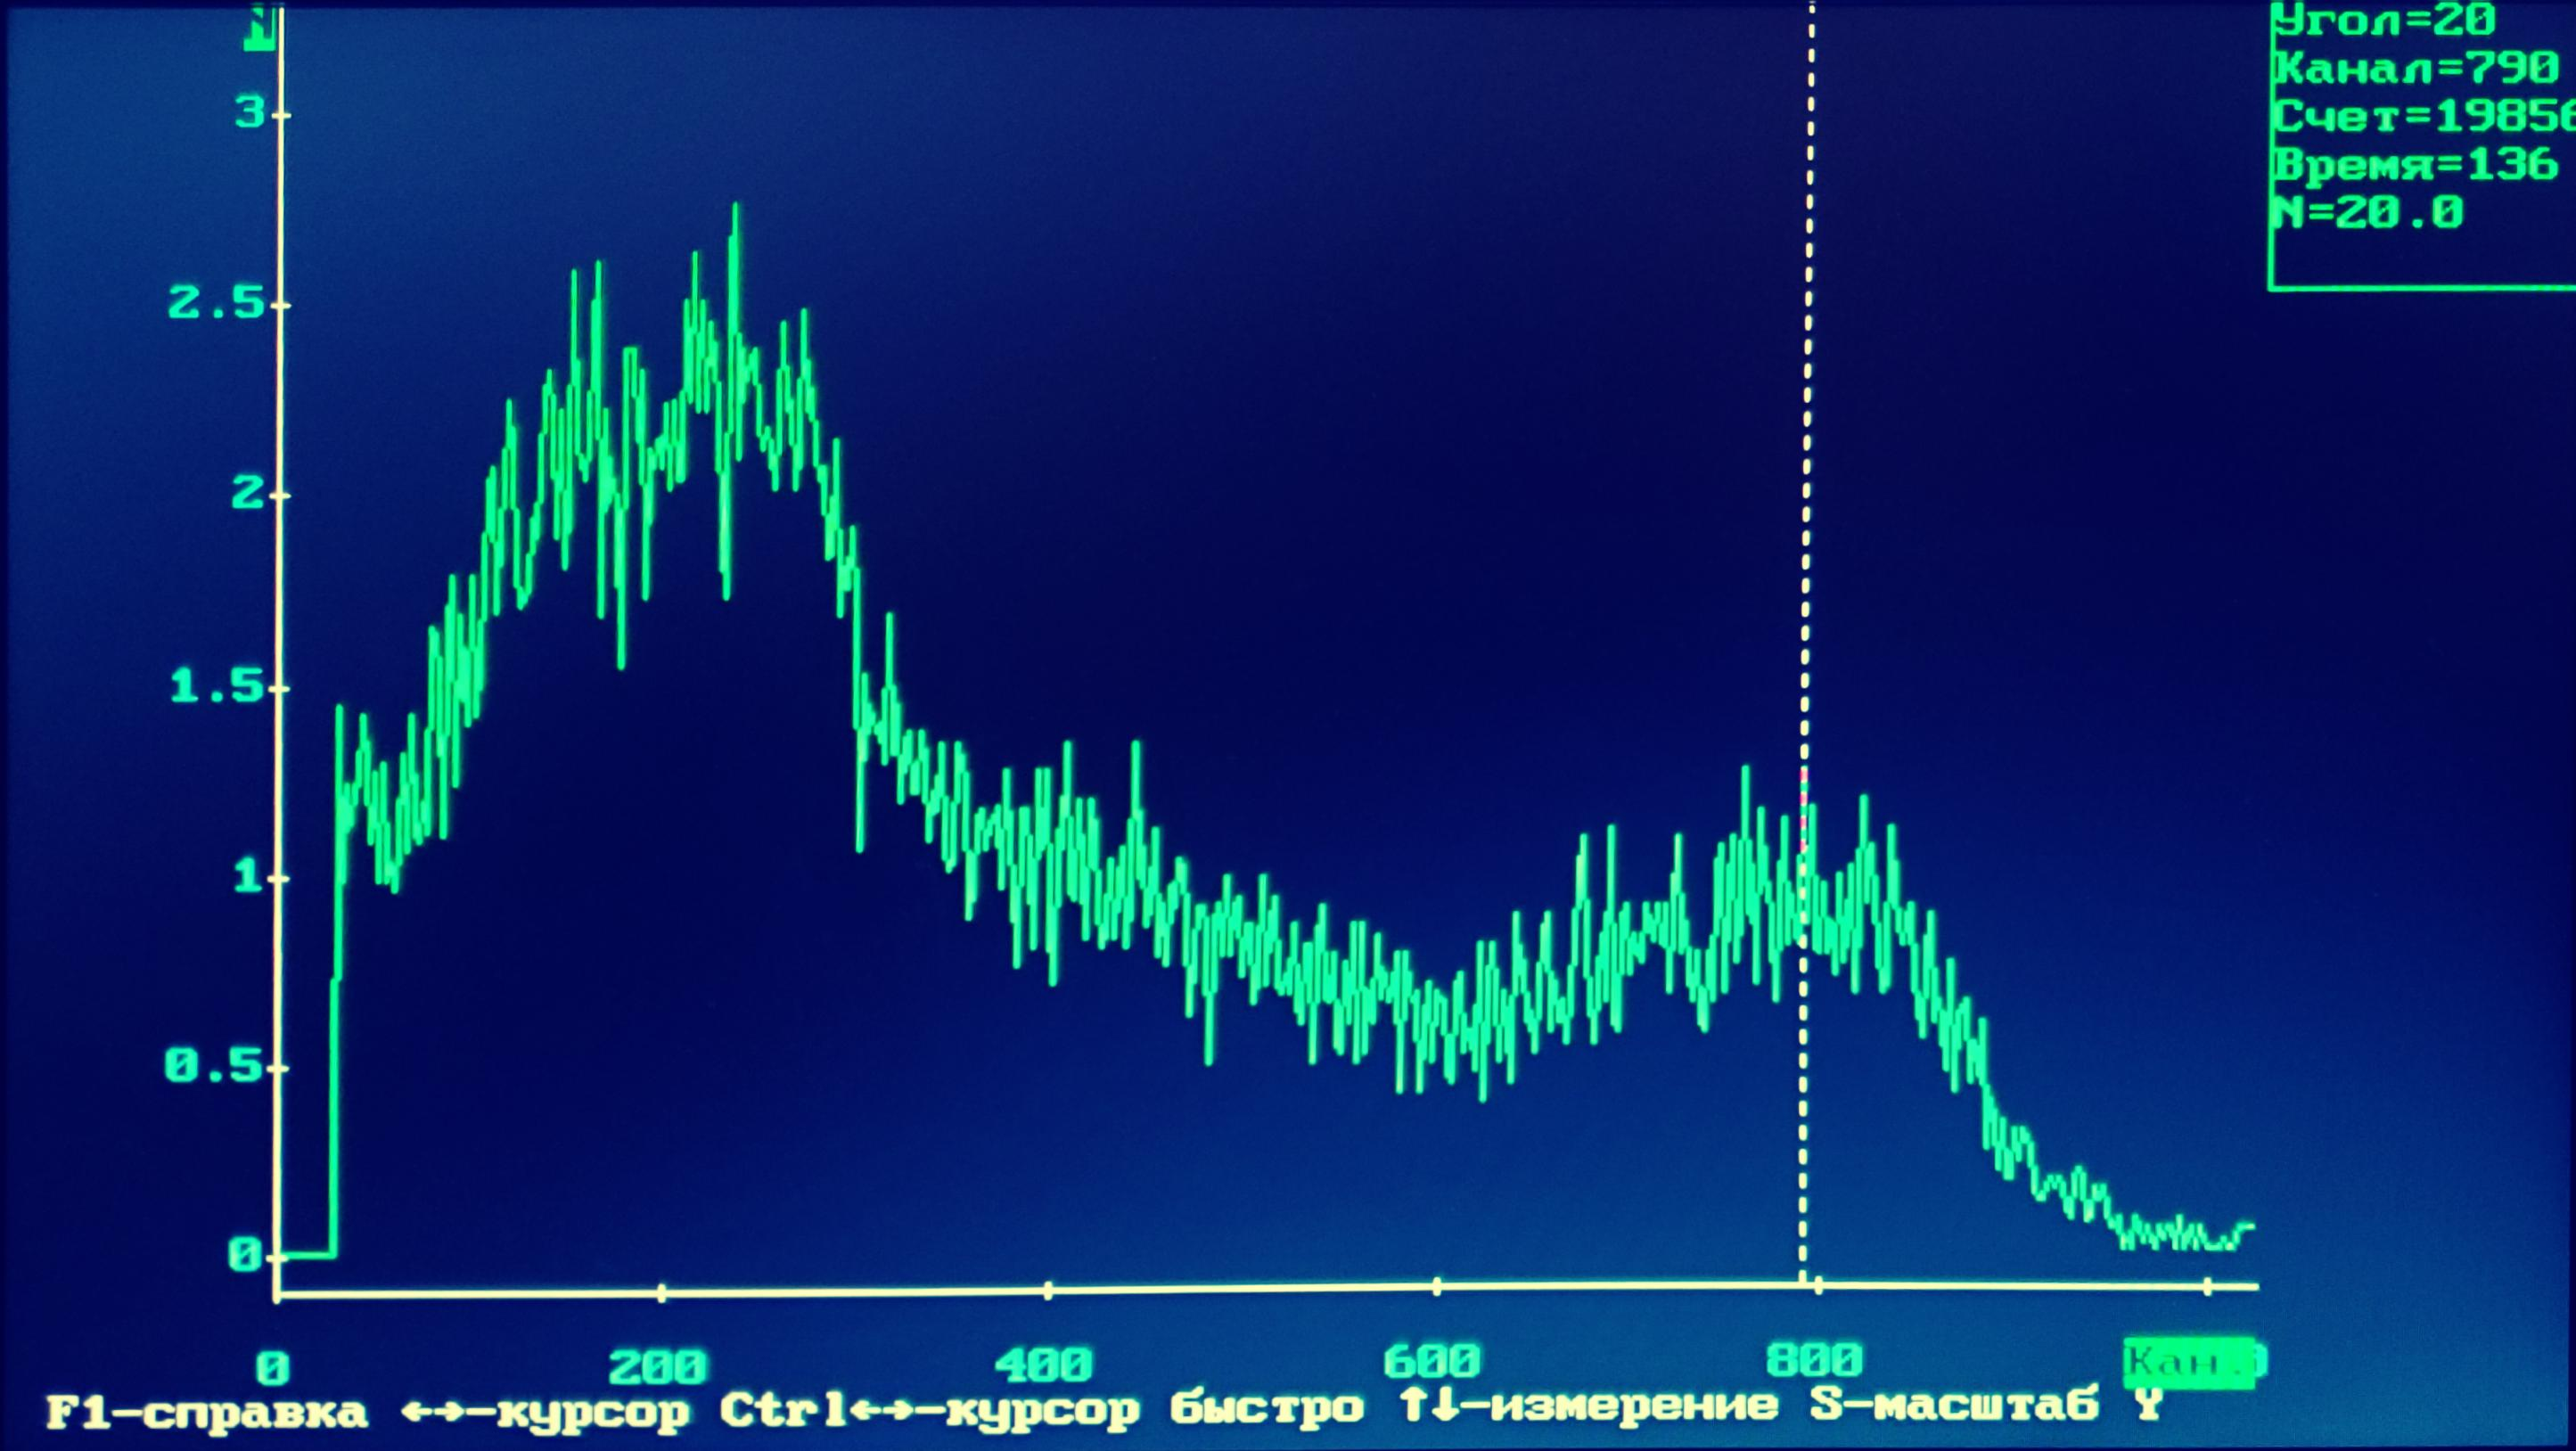
\includegraphics[width = \linewidth]{spectre20.jpg}}\\
      Рис 4. $\theta = 20^{\circ}$
    \end{minipage}
  \end{figure}
  \begin{figure}[h!]
    \begin{minipage}[h]{0.32\linewidth}
      \center{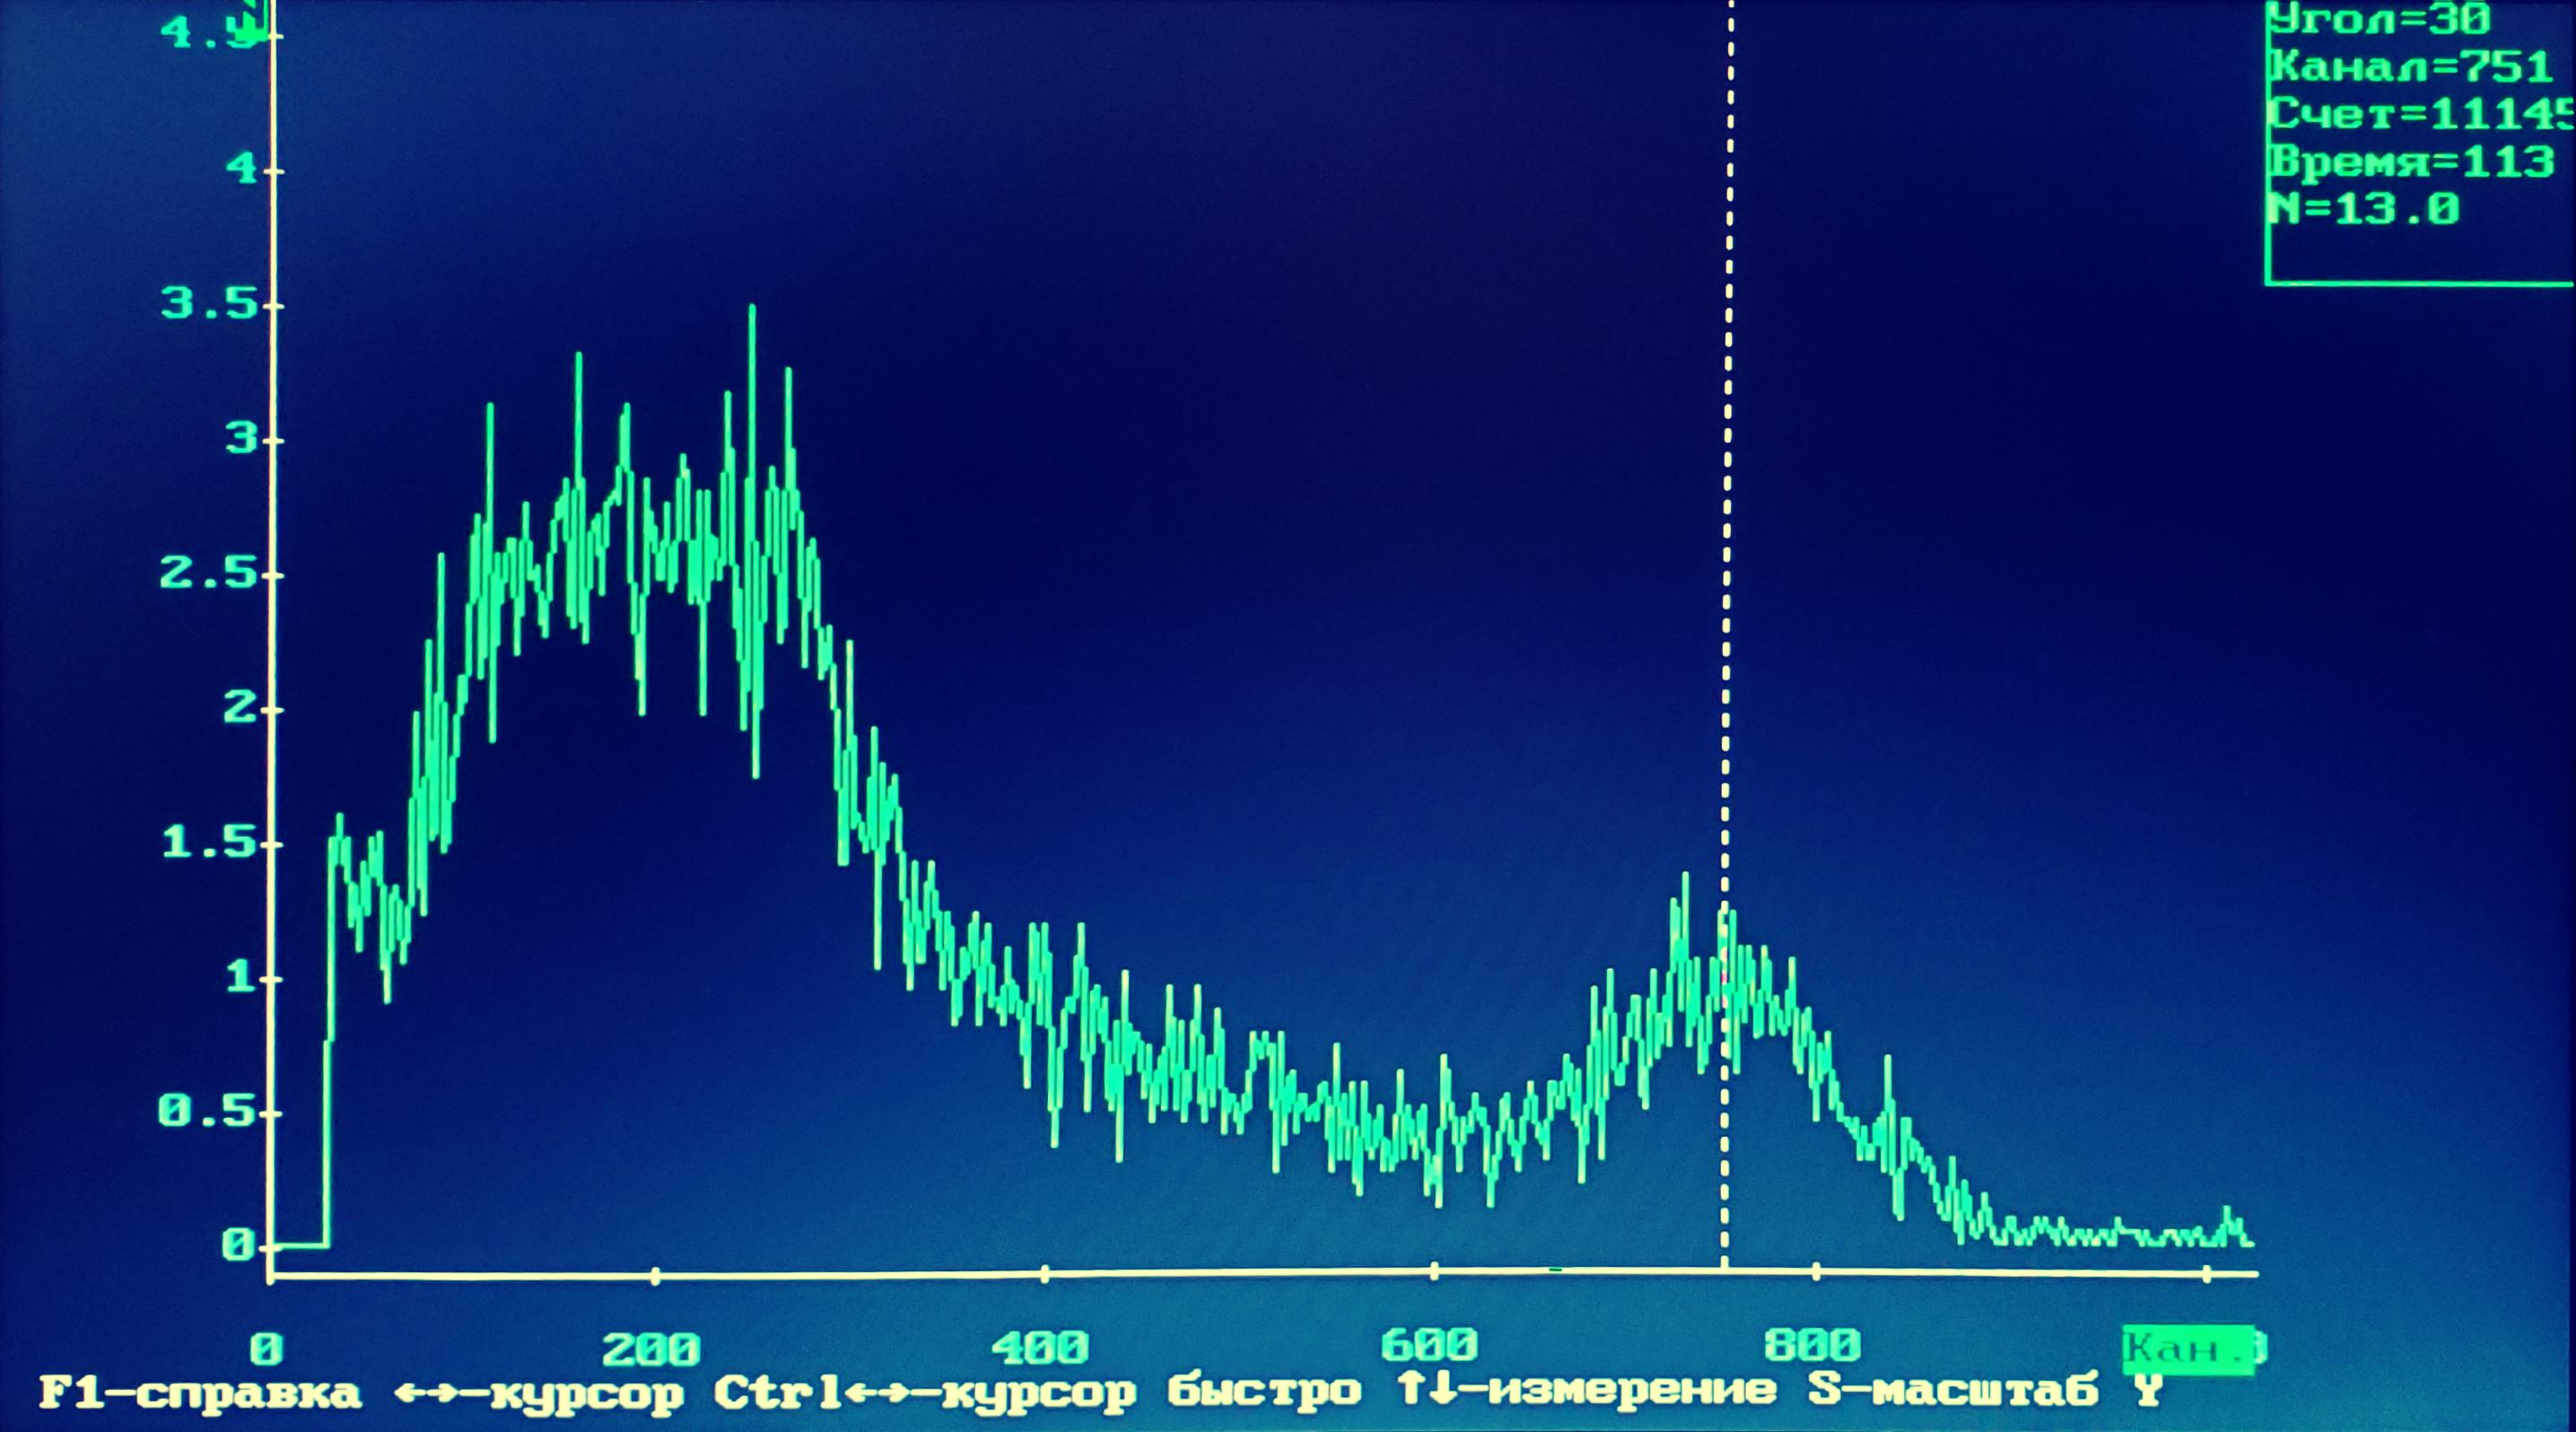
\includegraphics[width = \linewidth]{spectre30.jpg}}\\
      Рис 5. $\theta = 30^{\circ}$
    \end{minipage}
    \begin{minipage}[h]{0.32\linewidth}
      \center{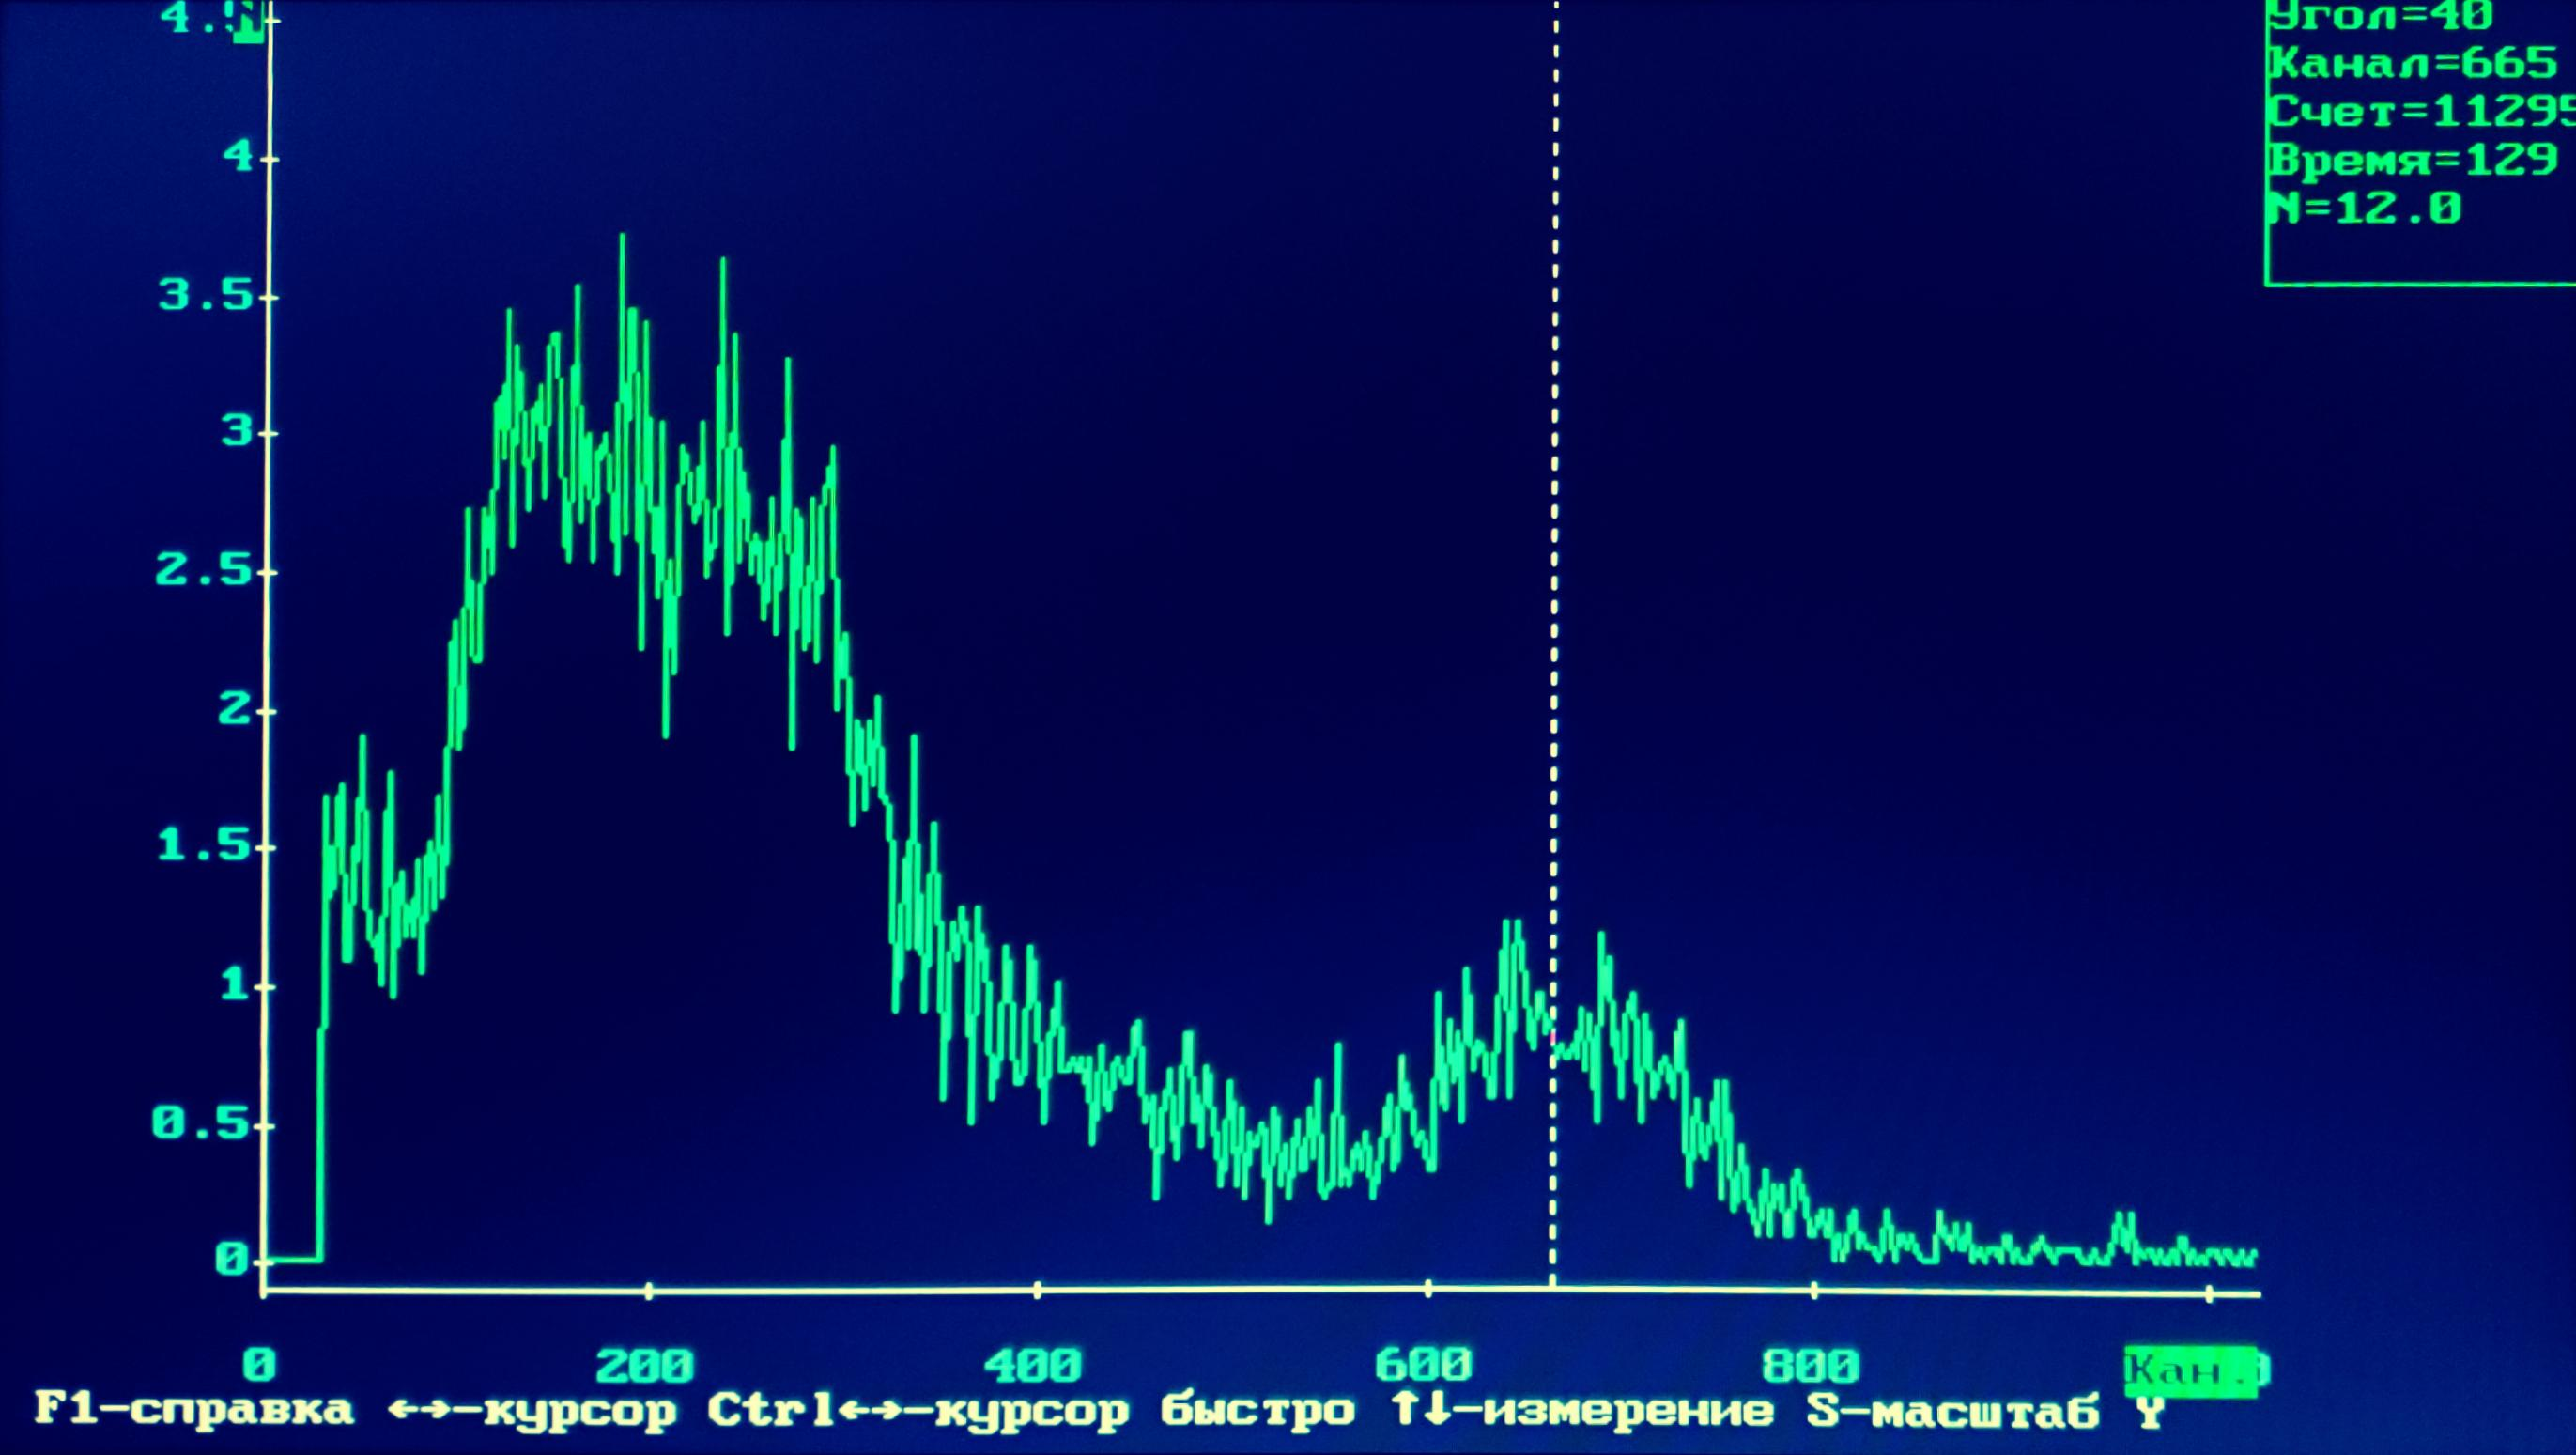
\includegraphics[width = \linewidth]{spectre40.jpg}}\\
      Рис 6. $\theta = 40^{\circ}$
    \end{minipage}
    \begin{minipage}[h]{0.32\linewidth}
      \center{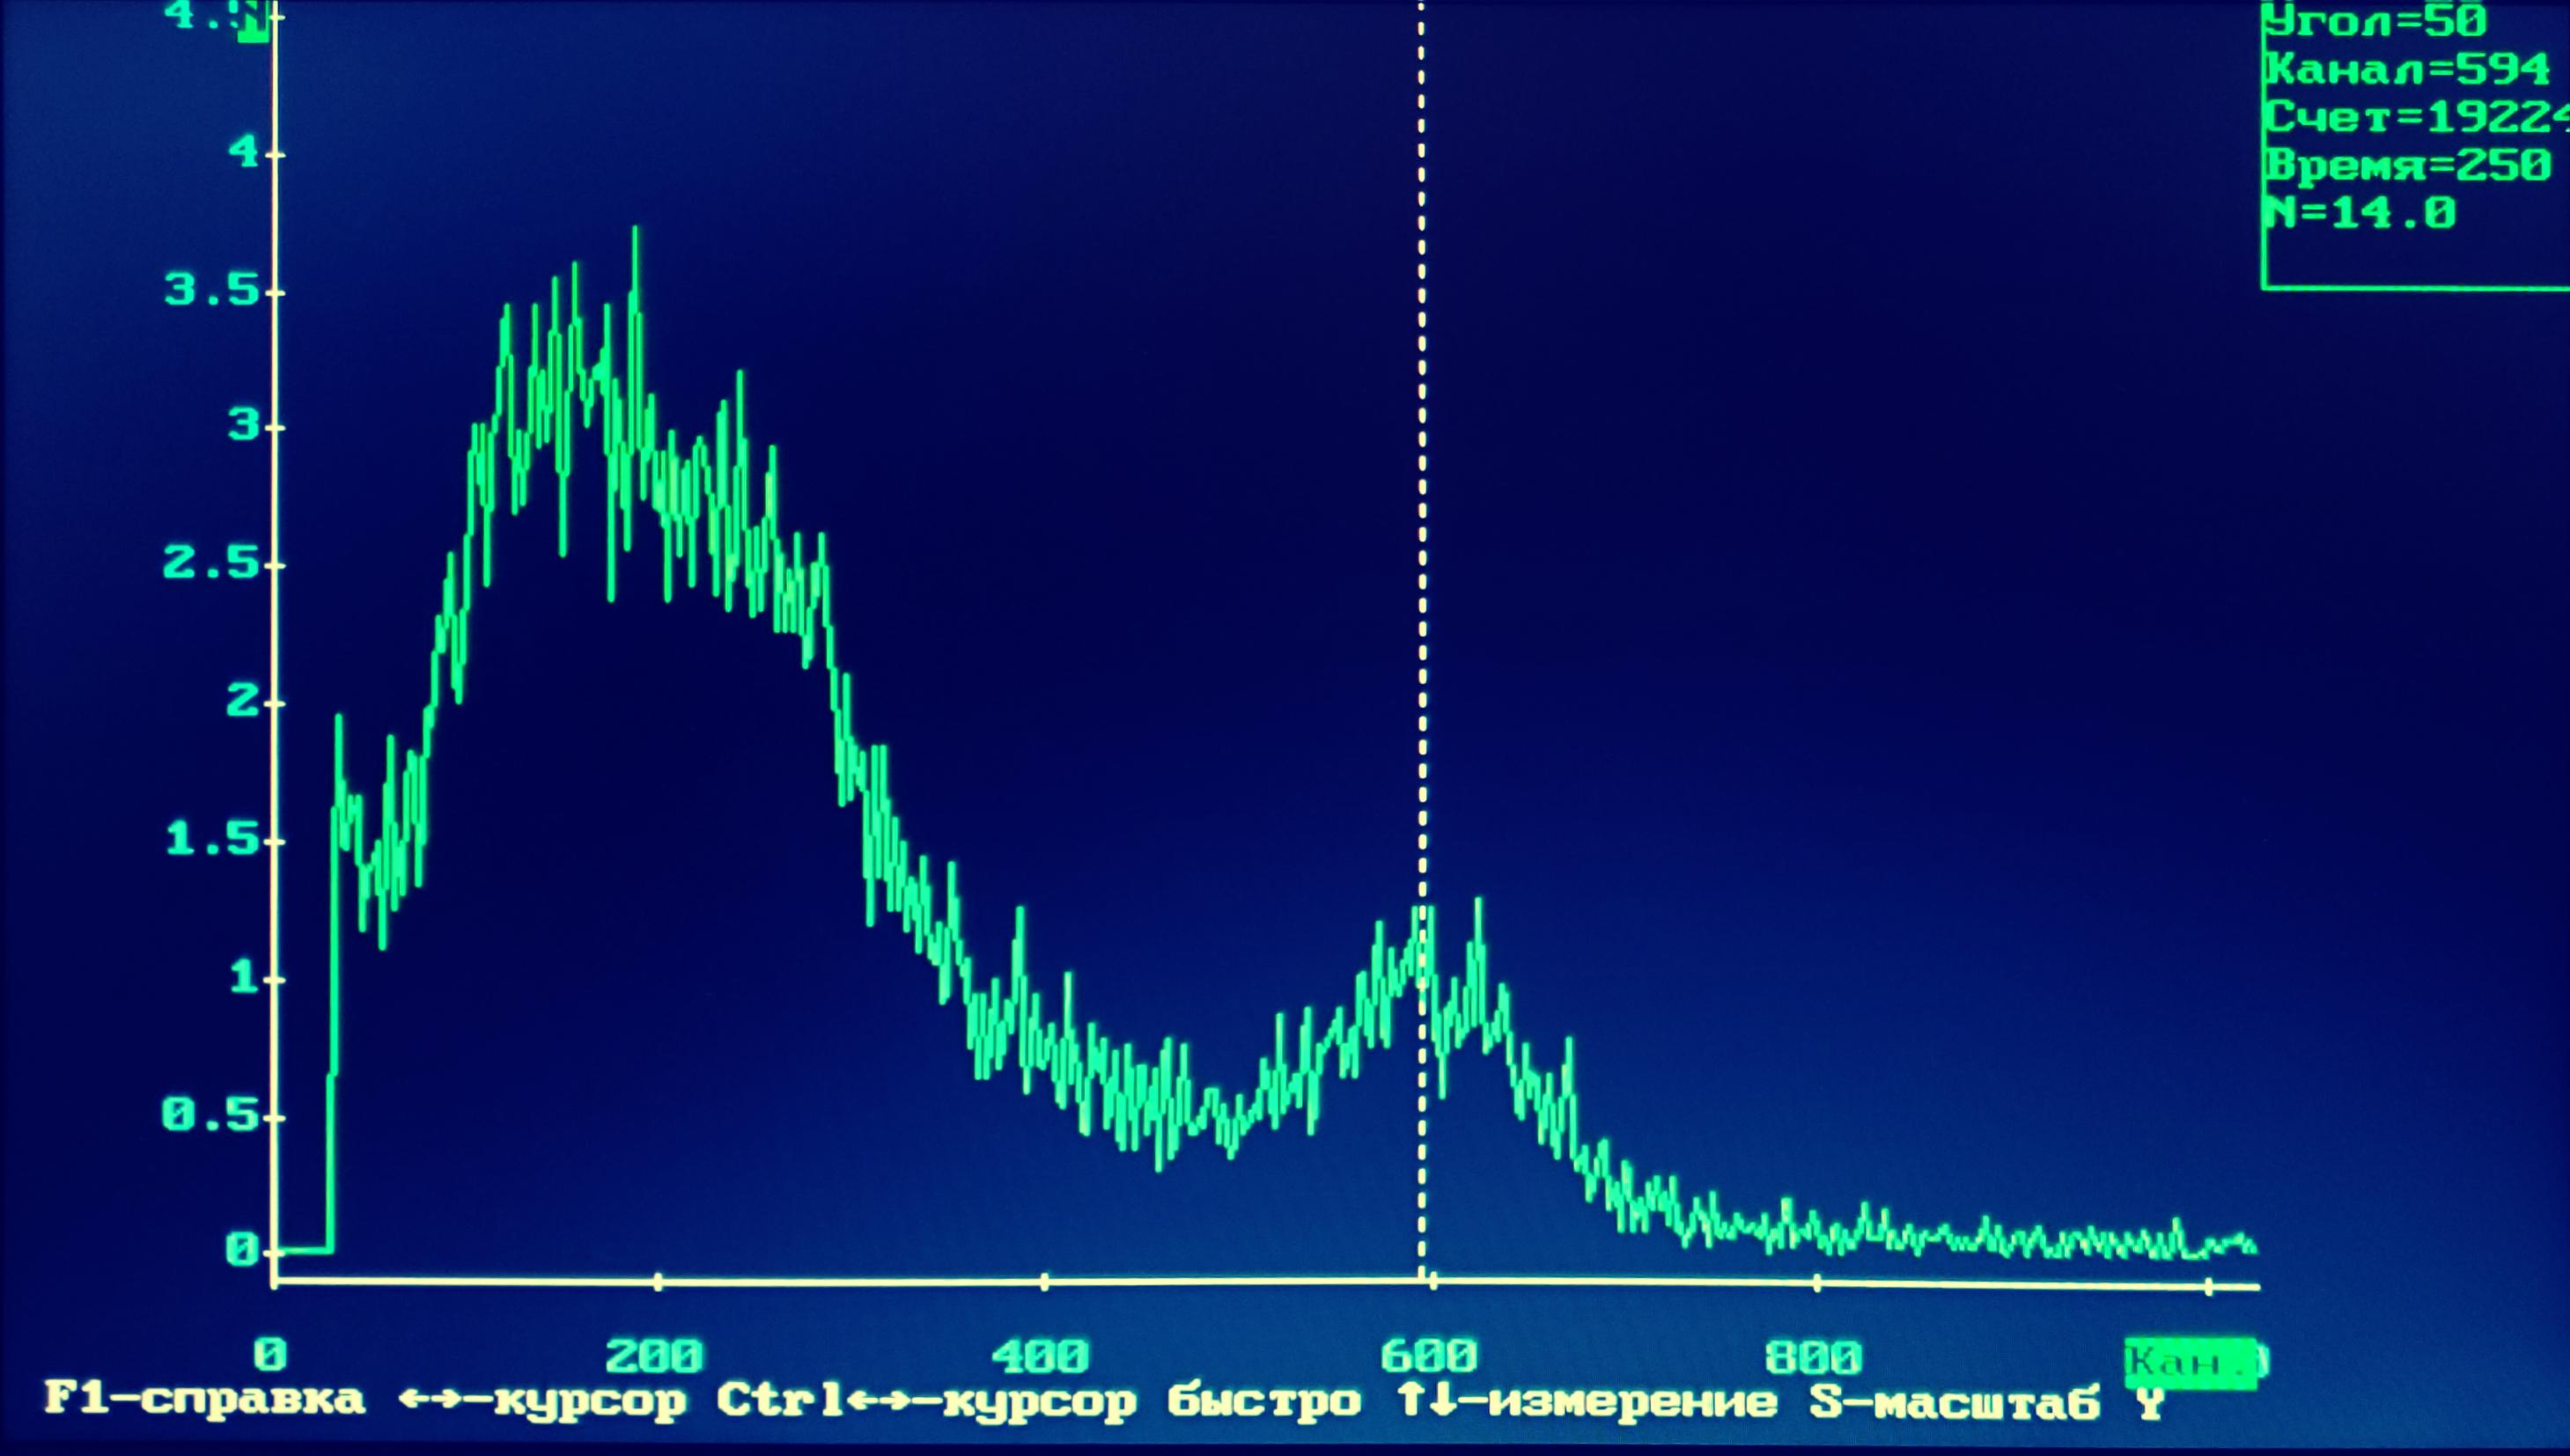
\includegraphics[width = \linewidth]{spectre50.jpg}}\\
      Рис 7. $\theta = 50^{\circ}$
    \end{minipage}
  \end{figure}
  \begin{figure}[h!]
    \begin{minipage}[h]{0.32\linewidth}
      \center{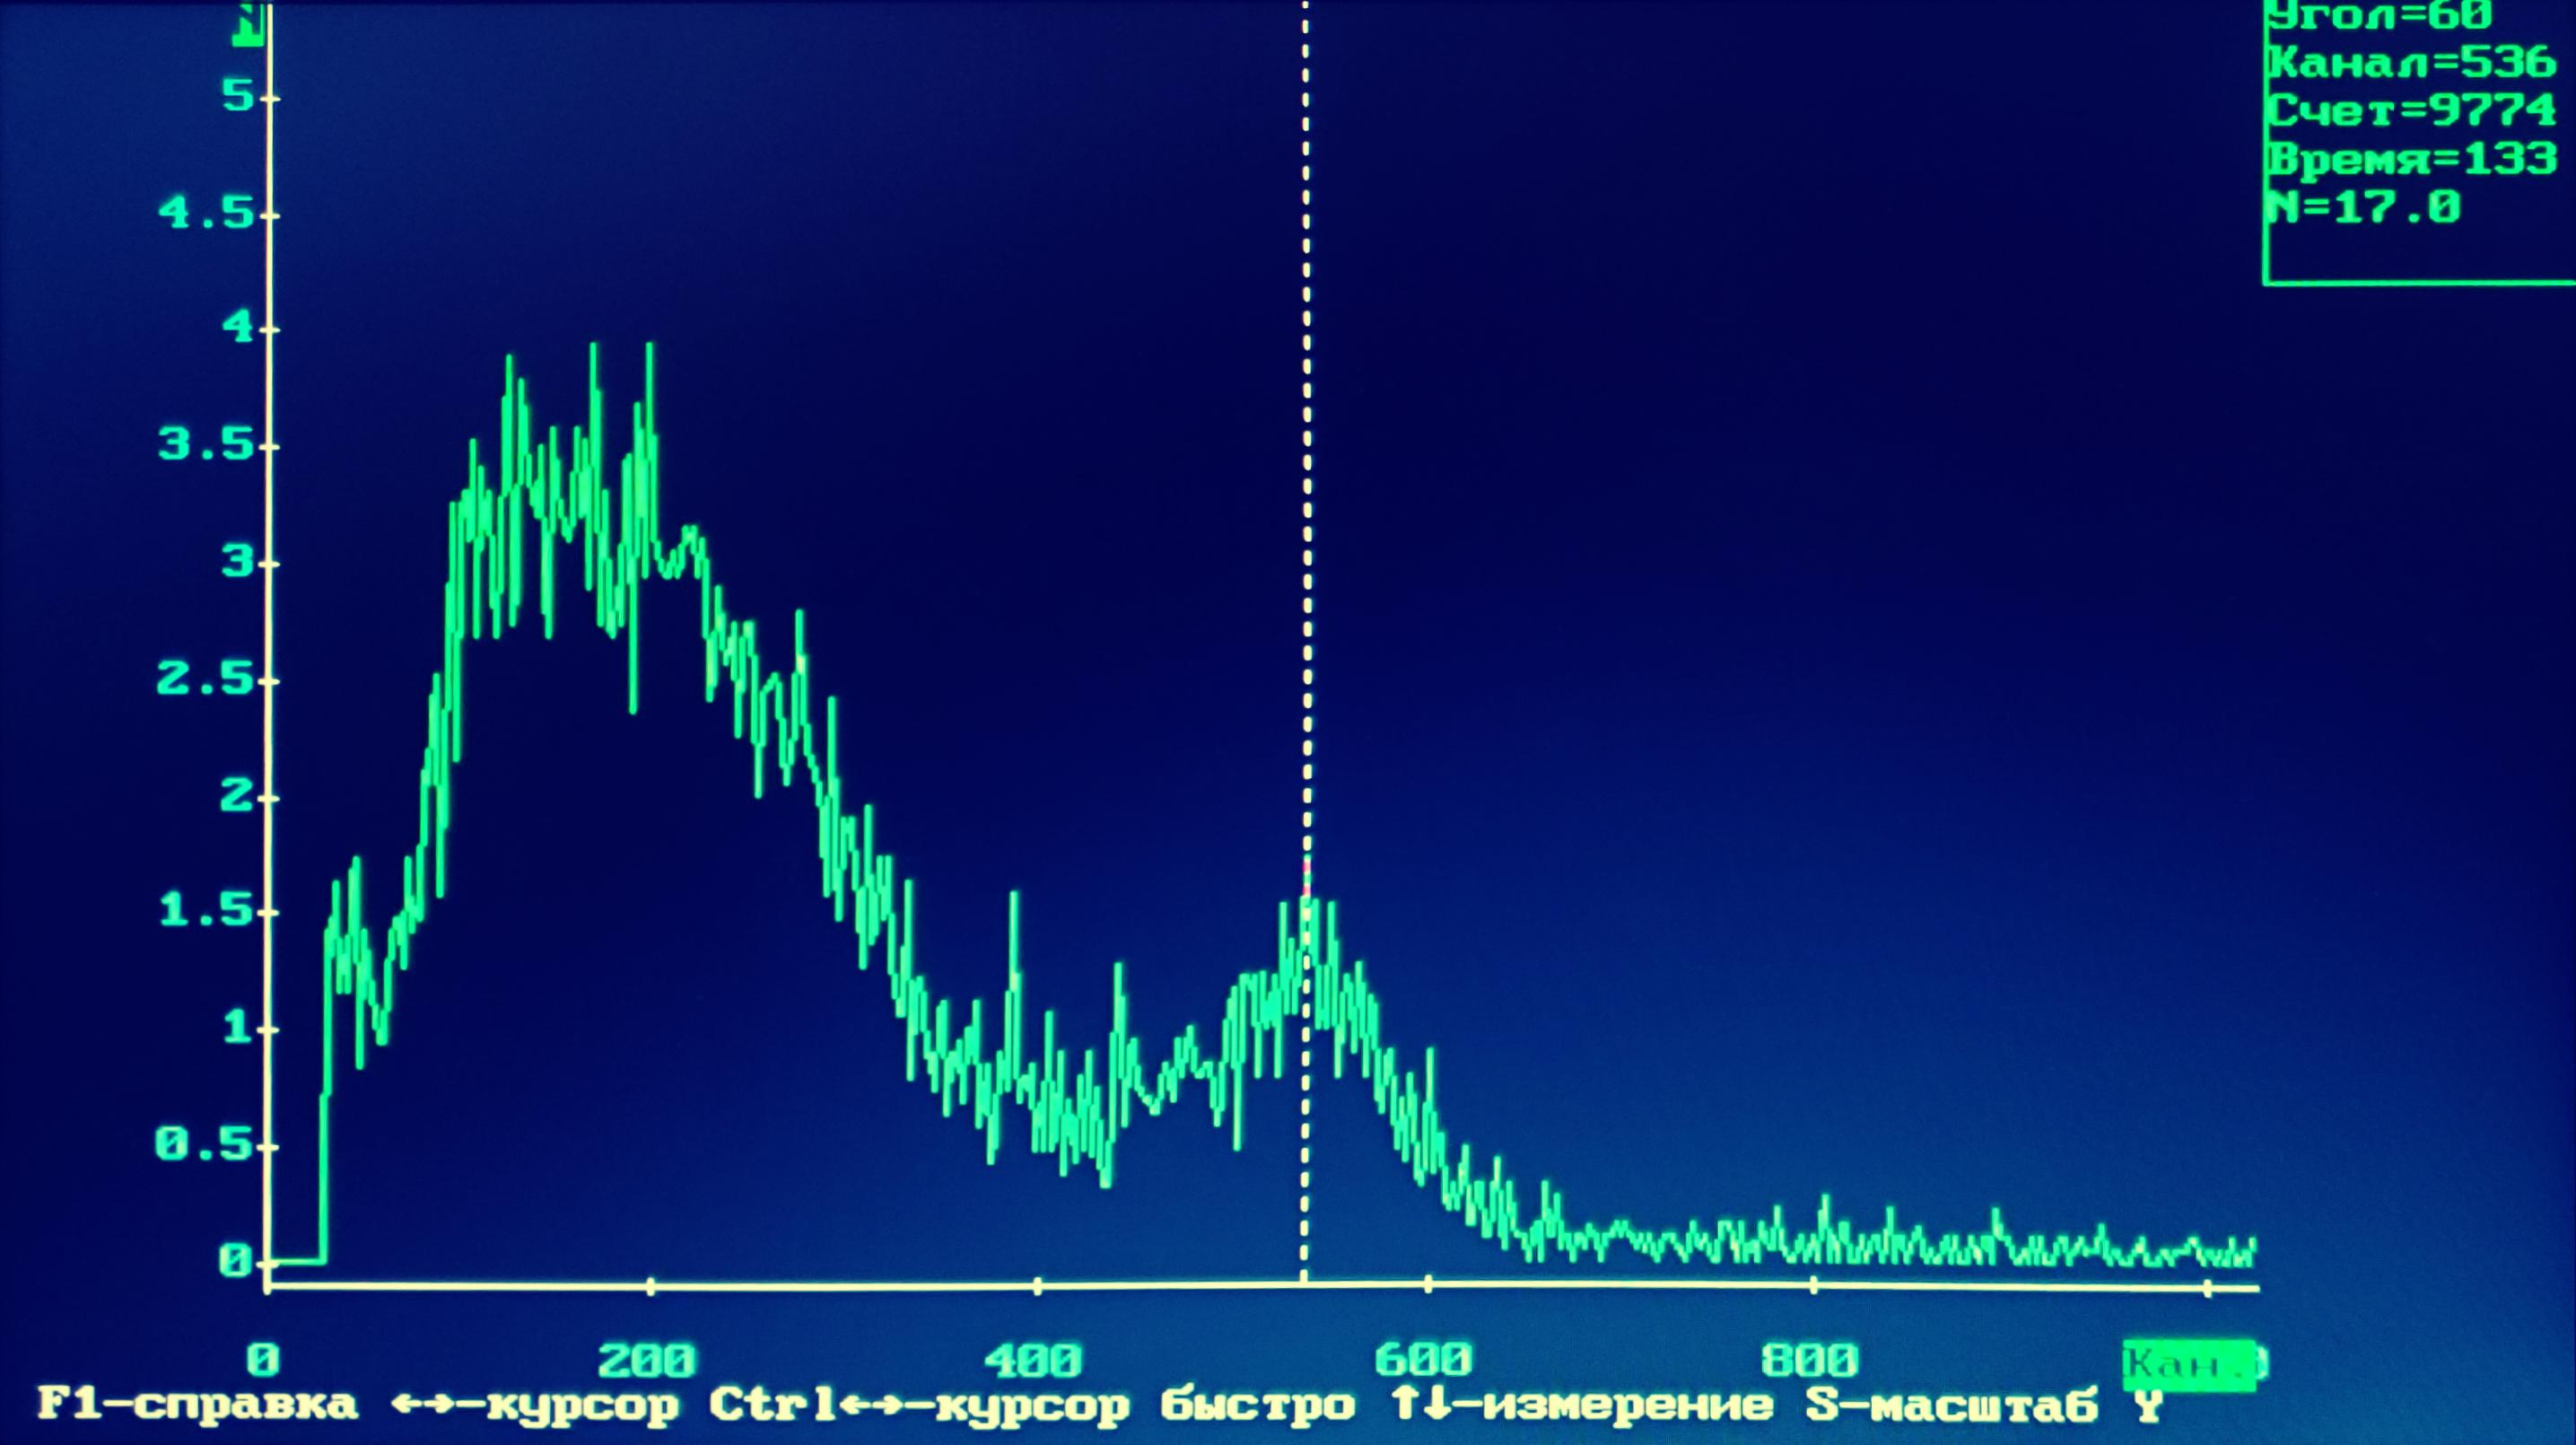
\includegraphics[width = \linewidth]{spectre60.jpg}}\\
      Рис 8. $\theta = 60^{\circ}$
    \end{minipage}
    \begin{minipage}[h]{0.32\linewidth}
      \center{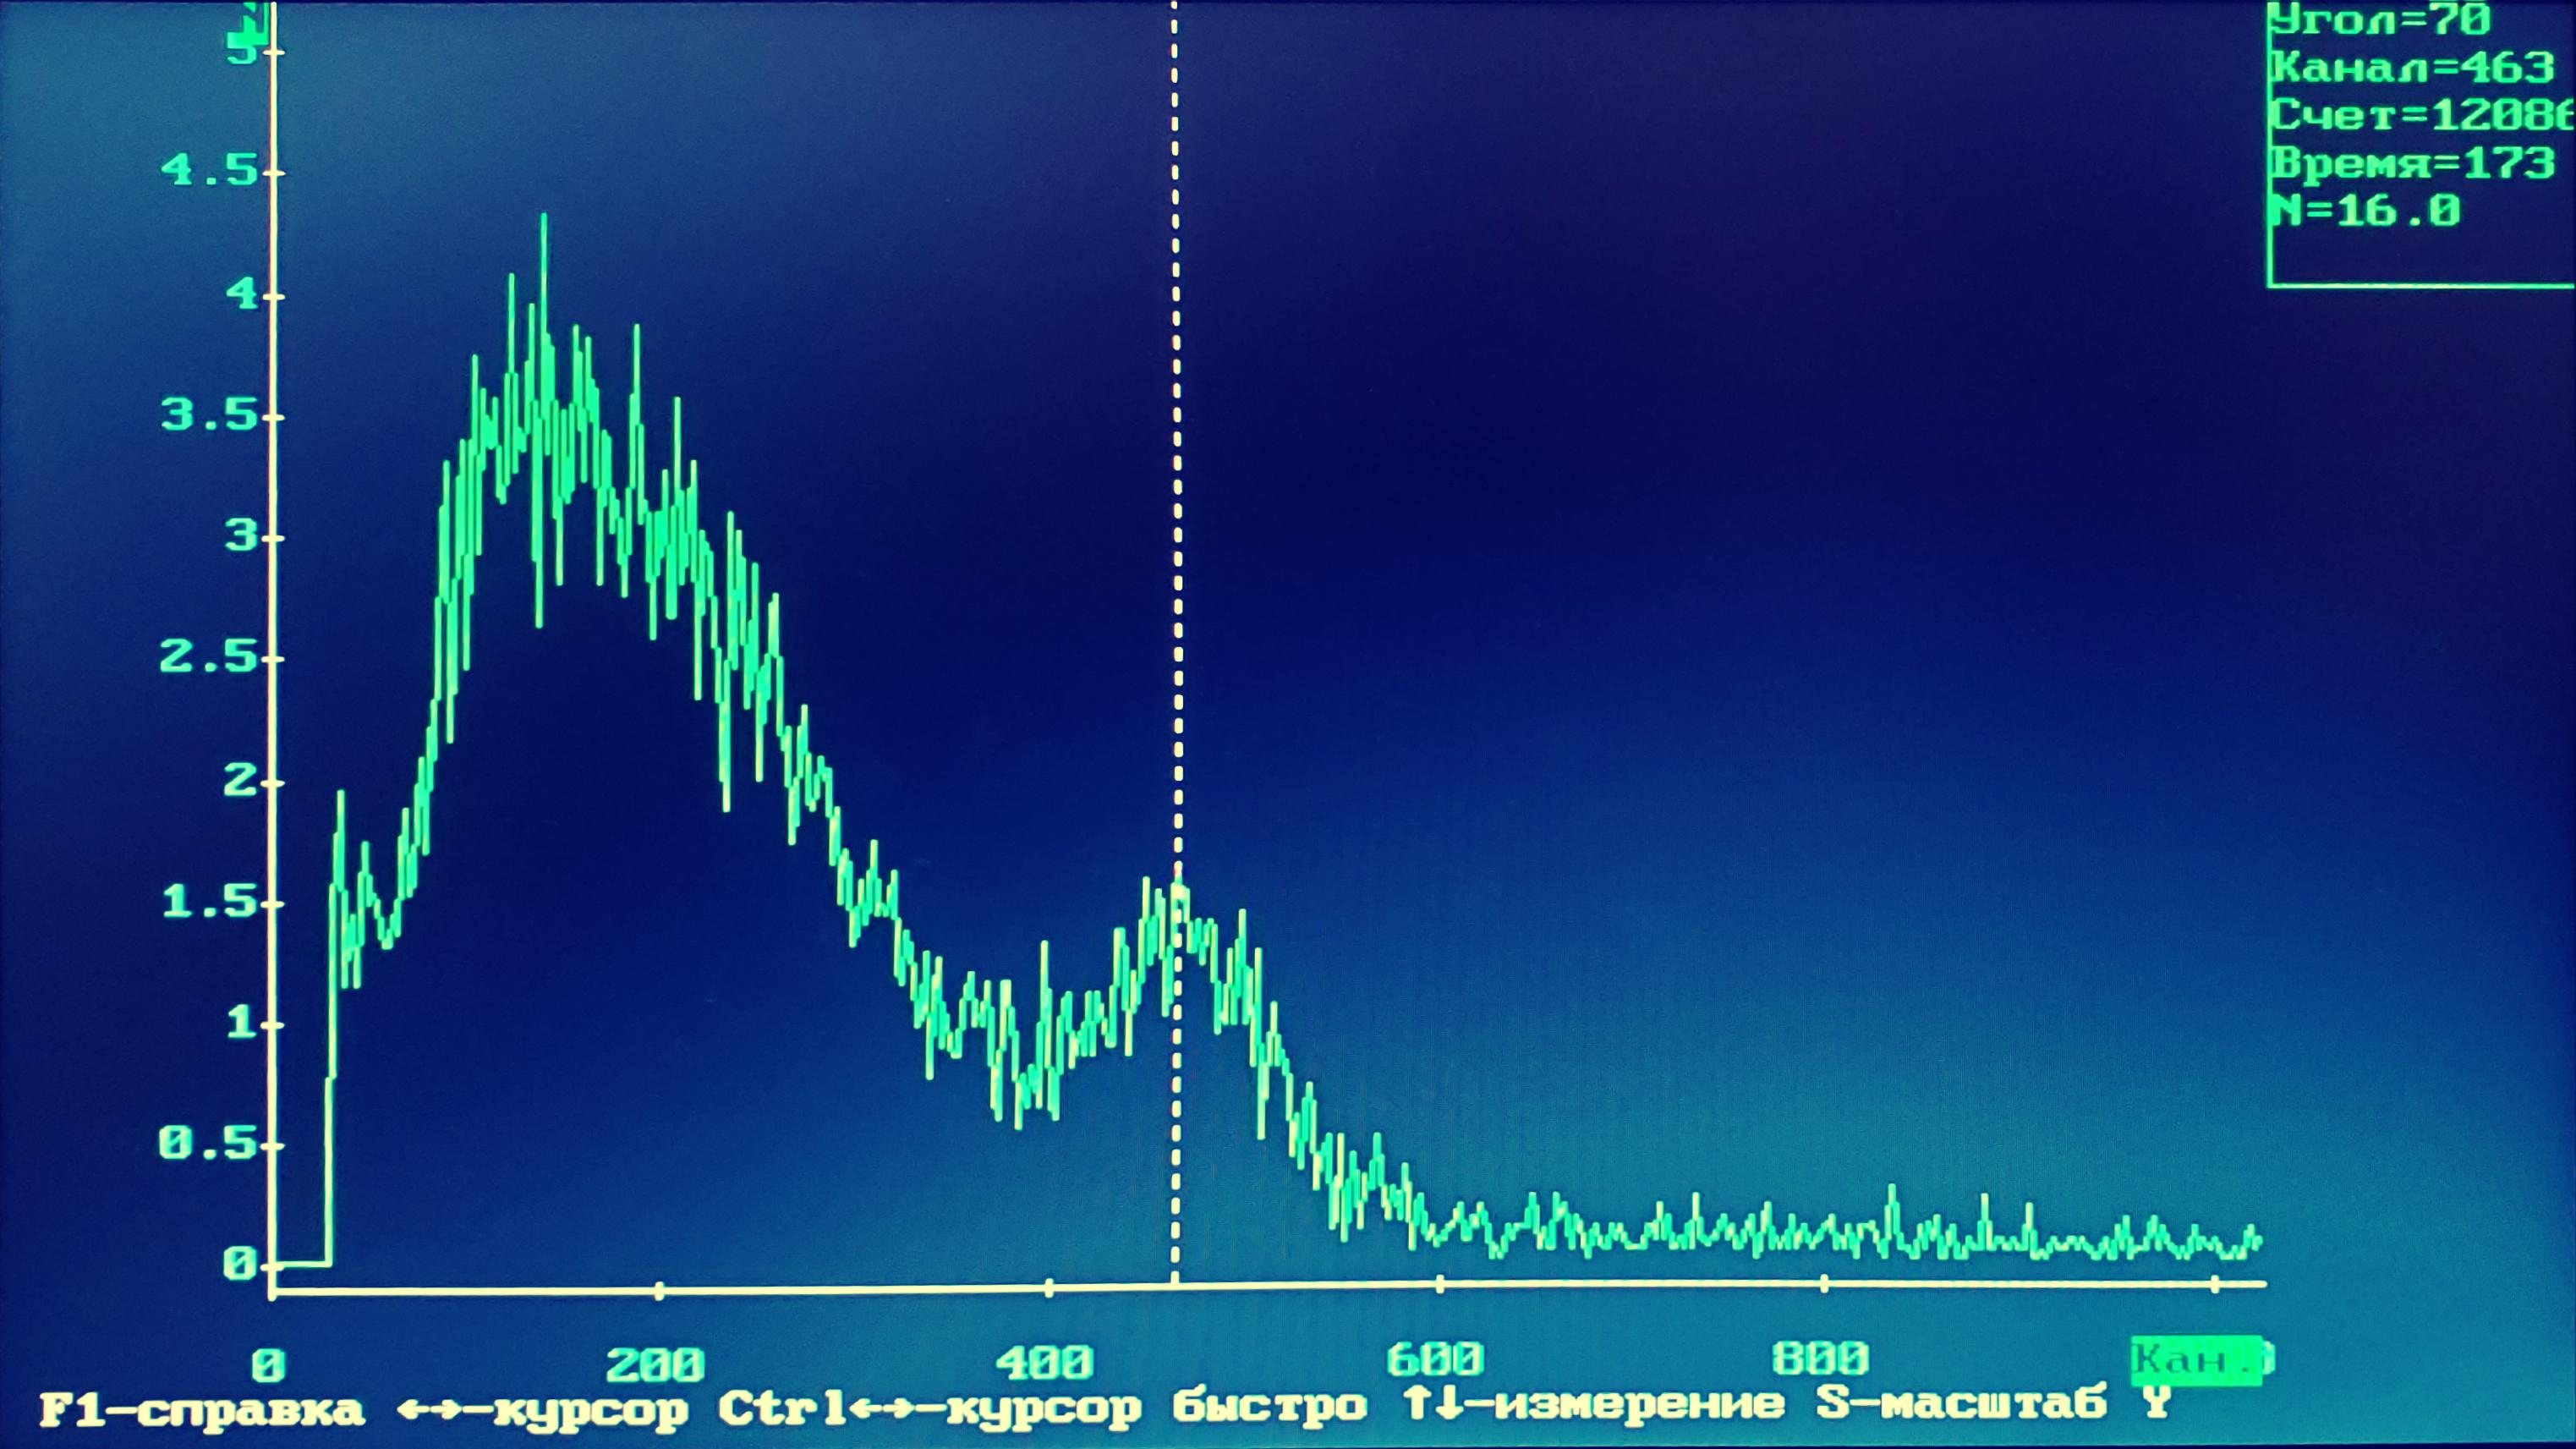
\includegraphics[width = \linewidth]{spectre70.jpg}}\\
      Рис 9. $\theta = 70^{\circ}$
    \end{minipage}
    \begin{minipage}[h]{0.32\linewidth}
      \center{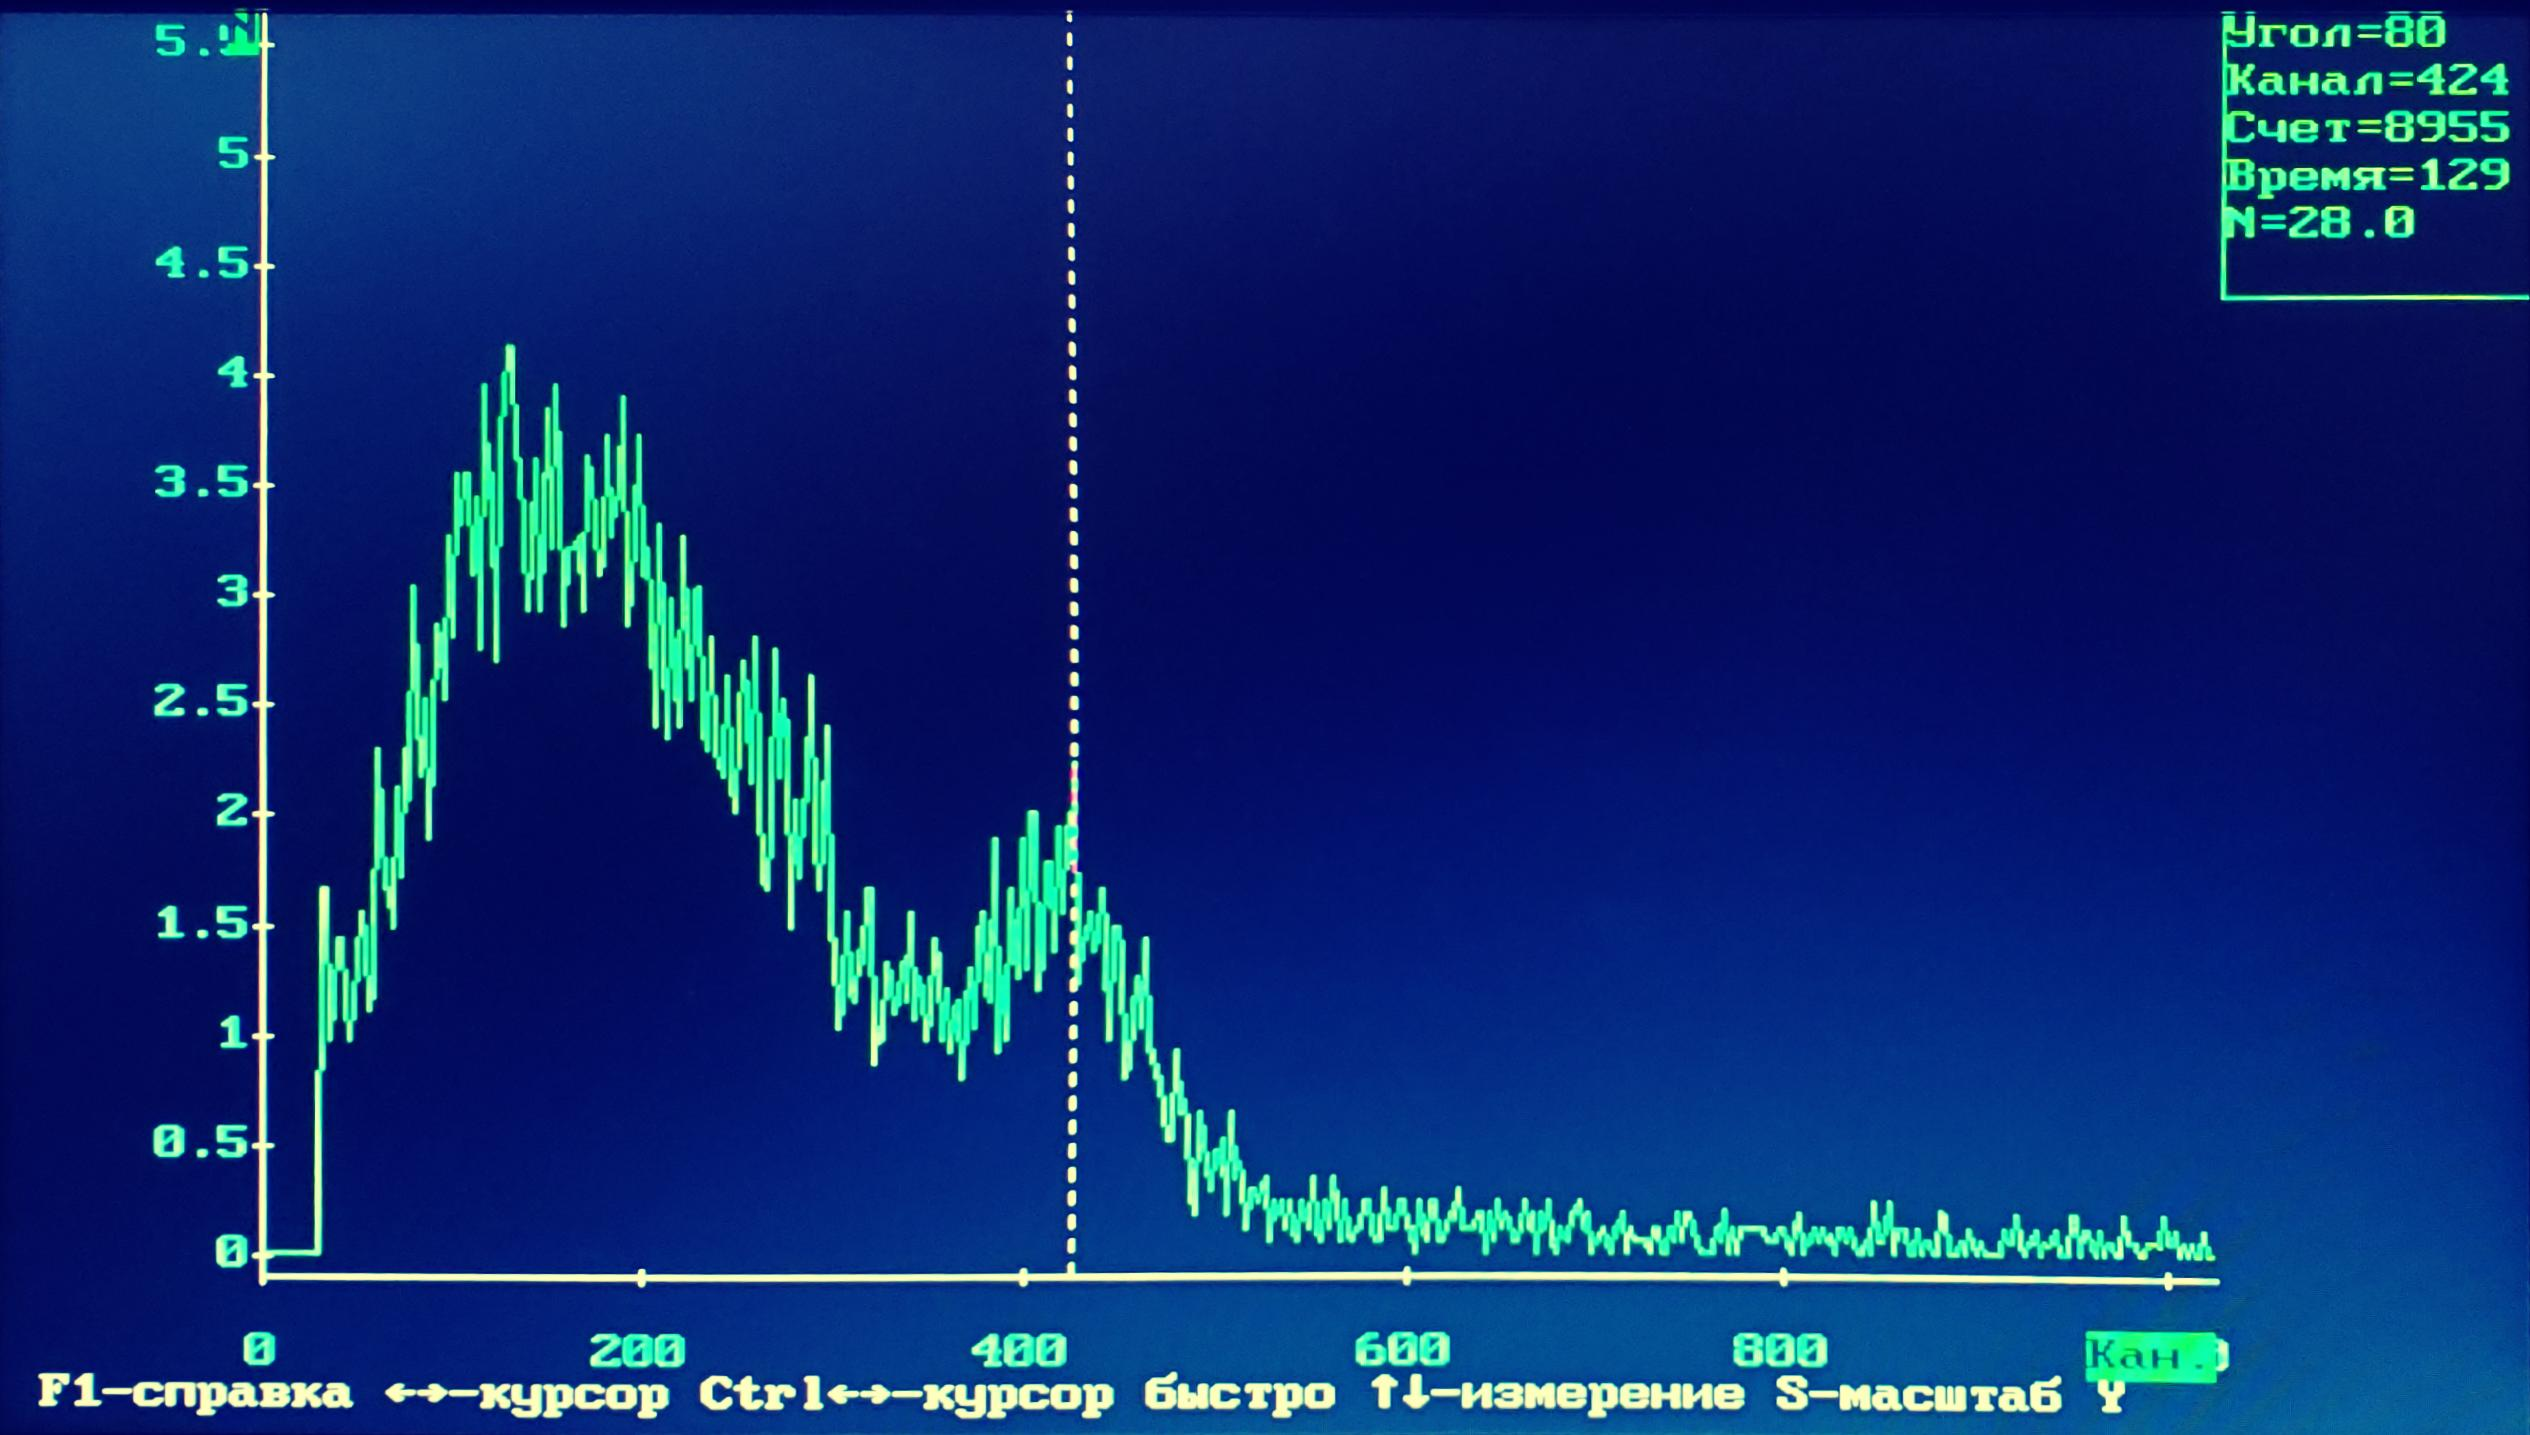
\includegraphics[width = \linewidth]{spectre80.jpg}}\\
      Рис 10. $\theta = 80^{\circ}$
    \end{minipage}
  \end{figure}
  \begin{figure}[h!]
    \begin{minipage}[h]{0.32\linewidth}
      \center{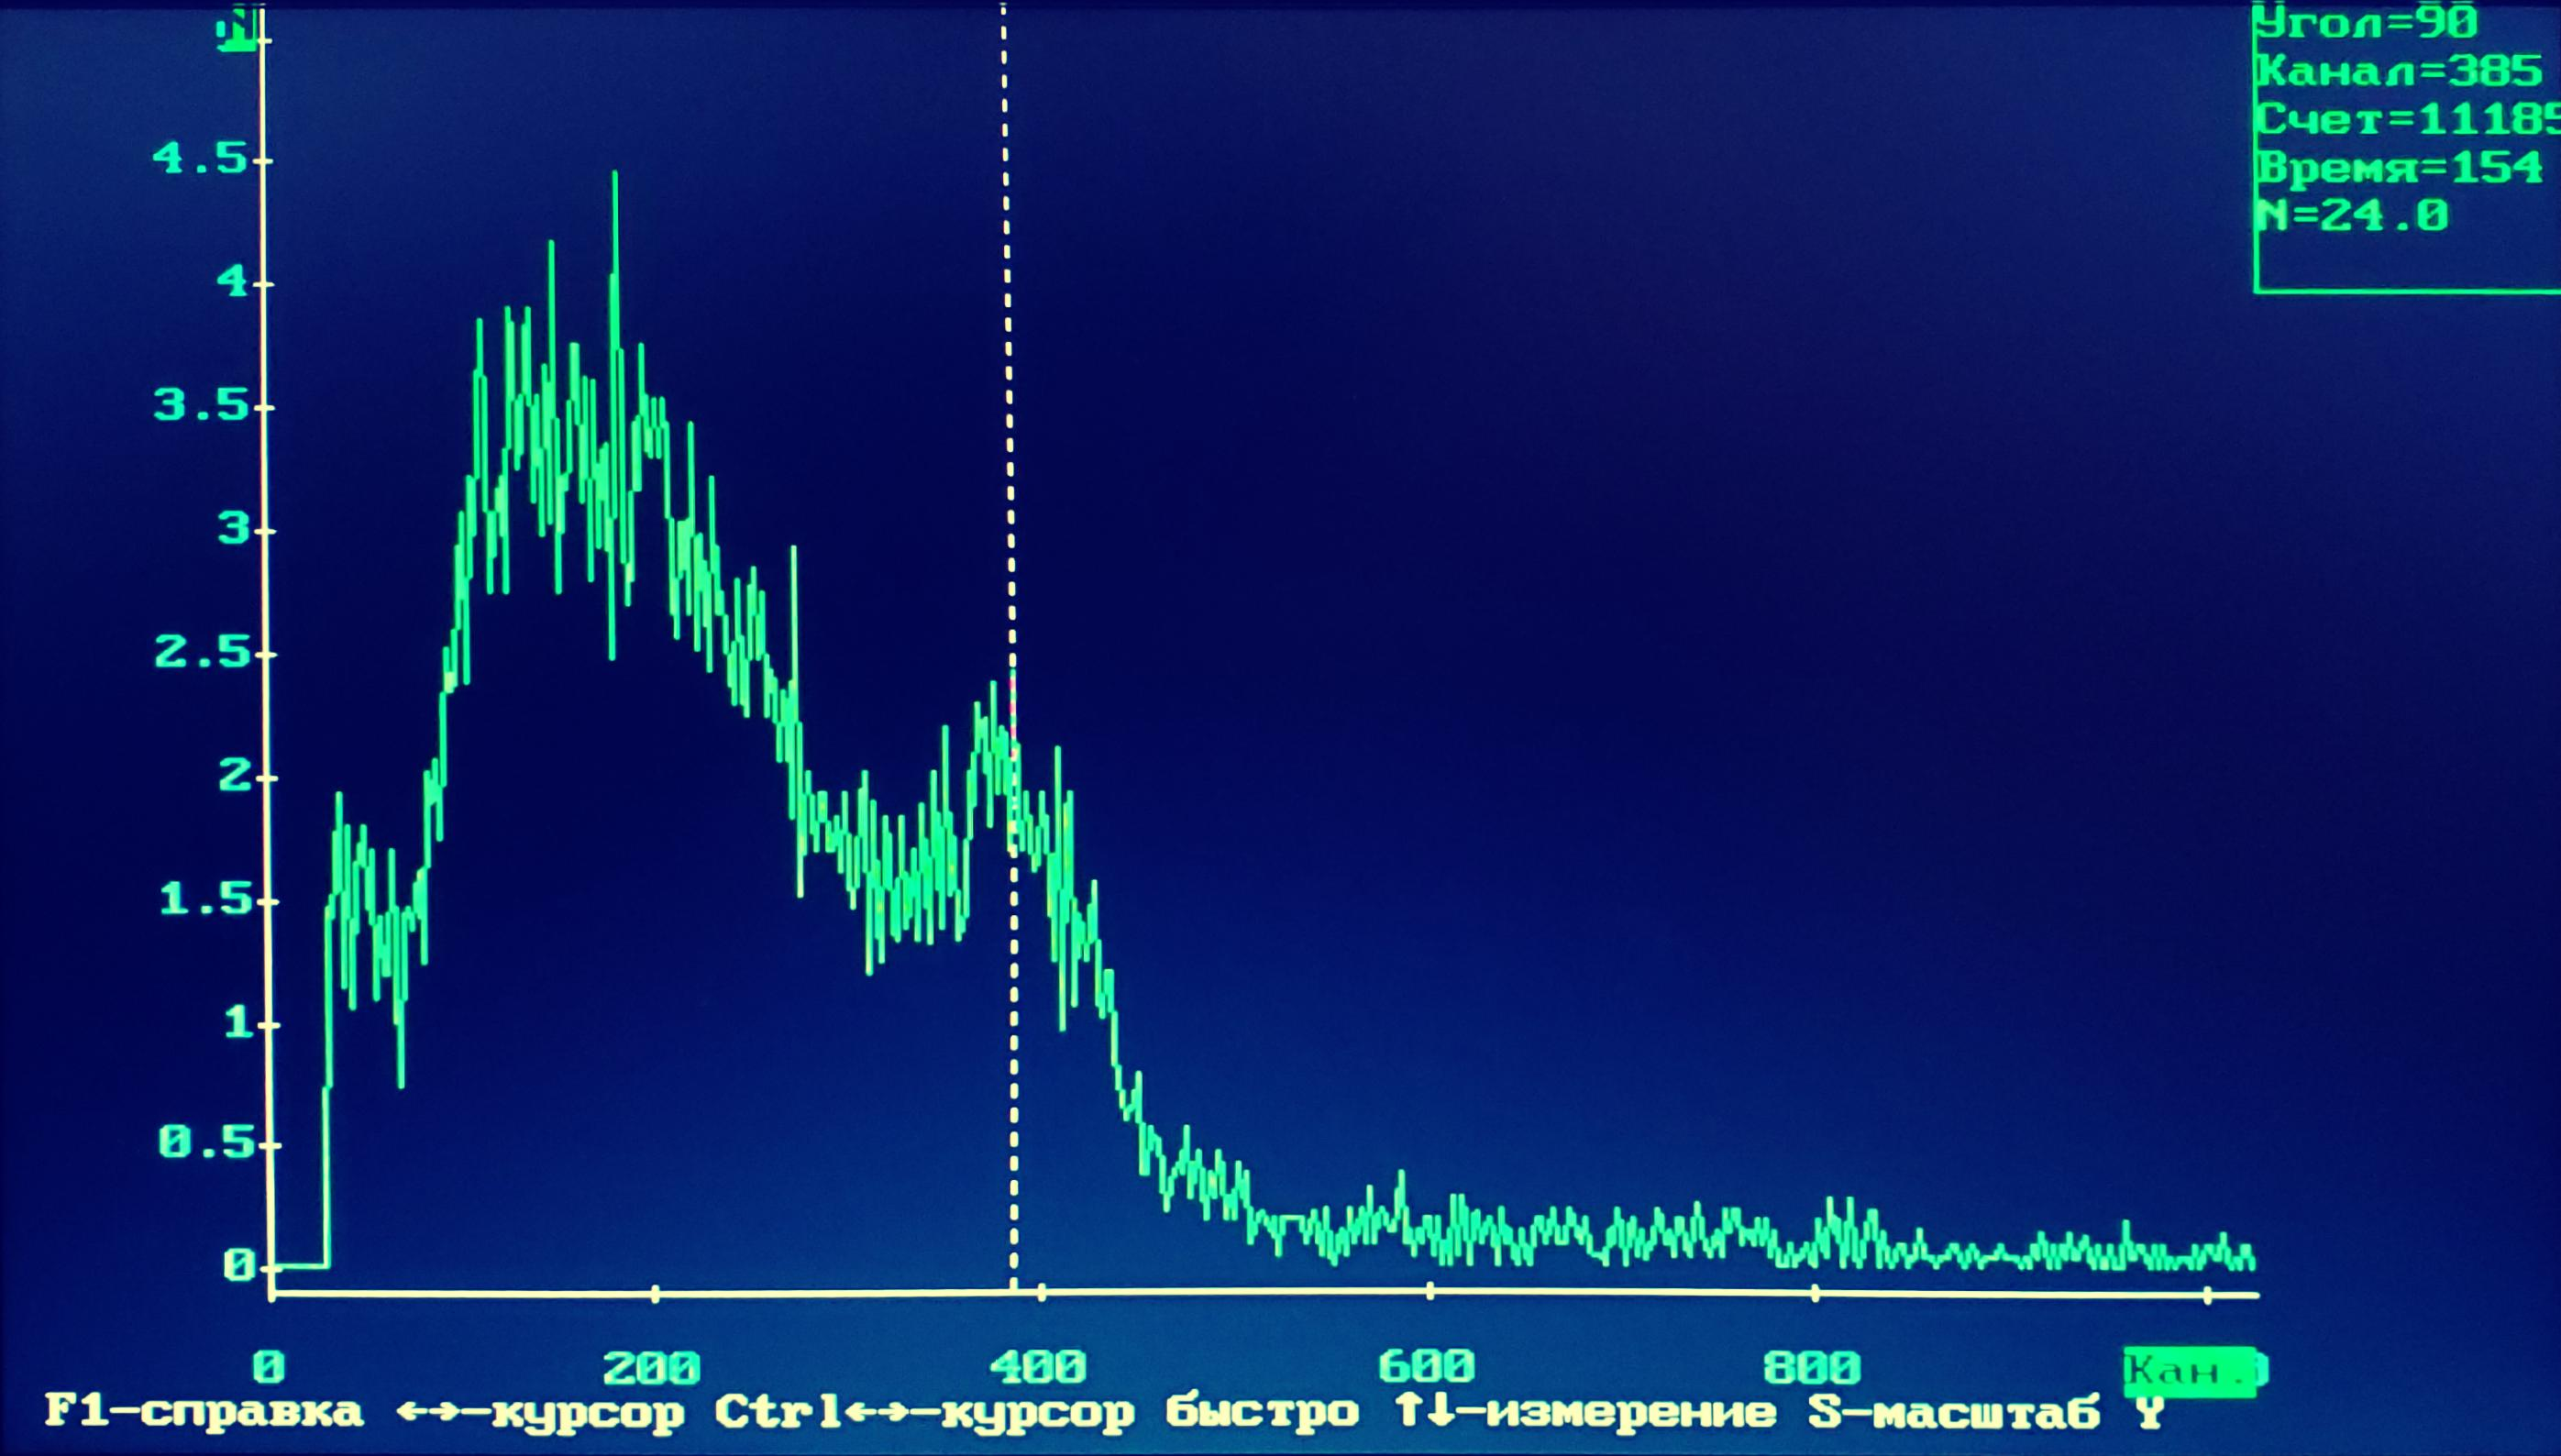
\includegraphics[width = \linewidth]{spectre90.jpg}}\\
      Рис 11. $\theta = 90^{\circ}$
    \end{minipage}
    \begin{minipage}[h]{0.32\linewidth}
      \center{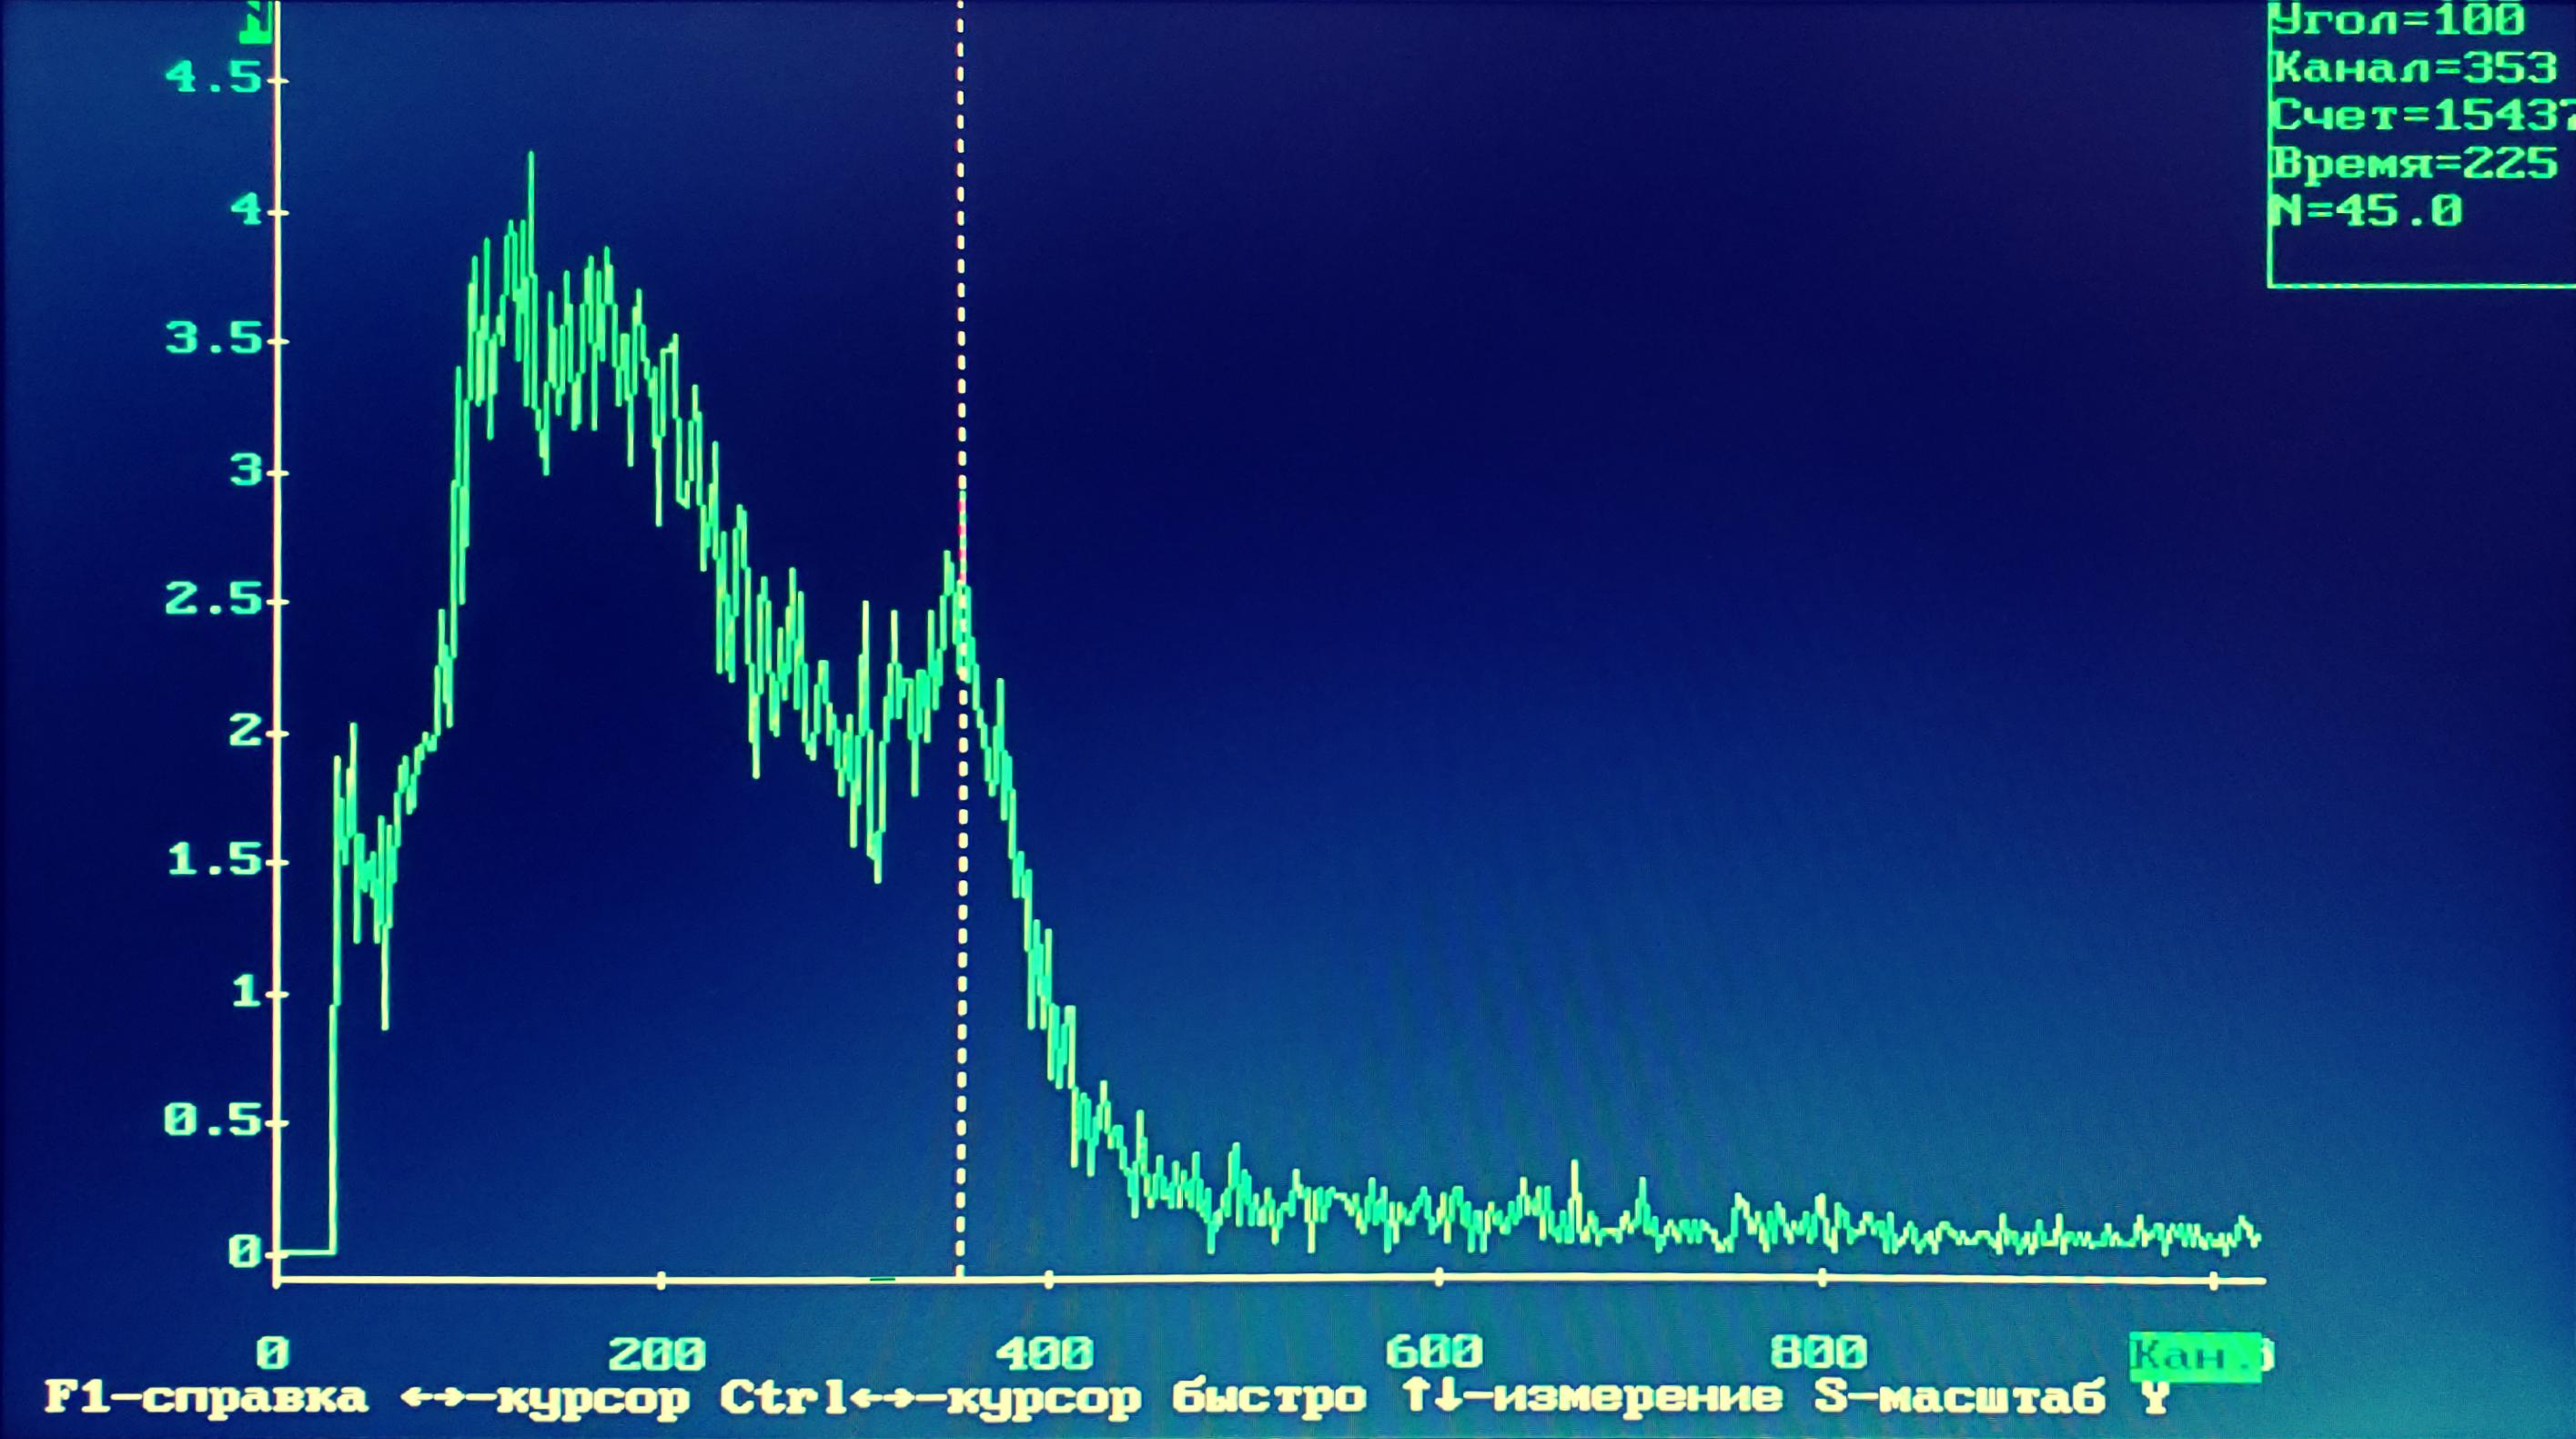
\includegraphics[width = \linewidth]{spectre100.jpg}}\\
      Рис 12. $\theta = 100^{\circ}$
    \end{minipage}
    \begin{minipage}[h]{0.32\linewidth}
      \center{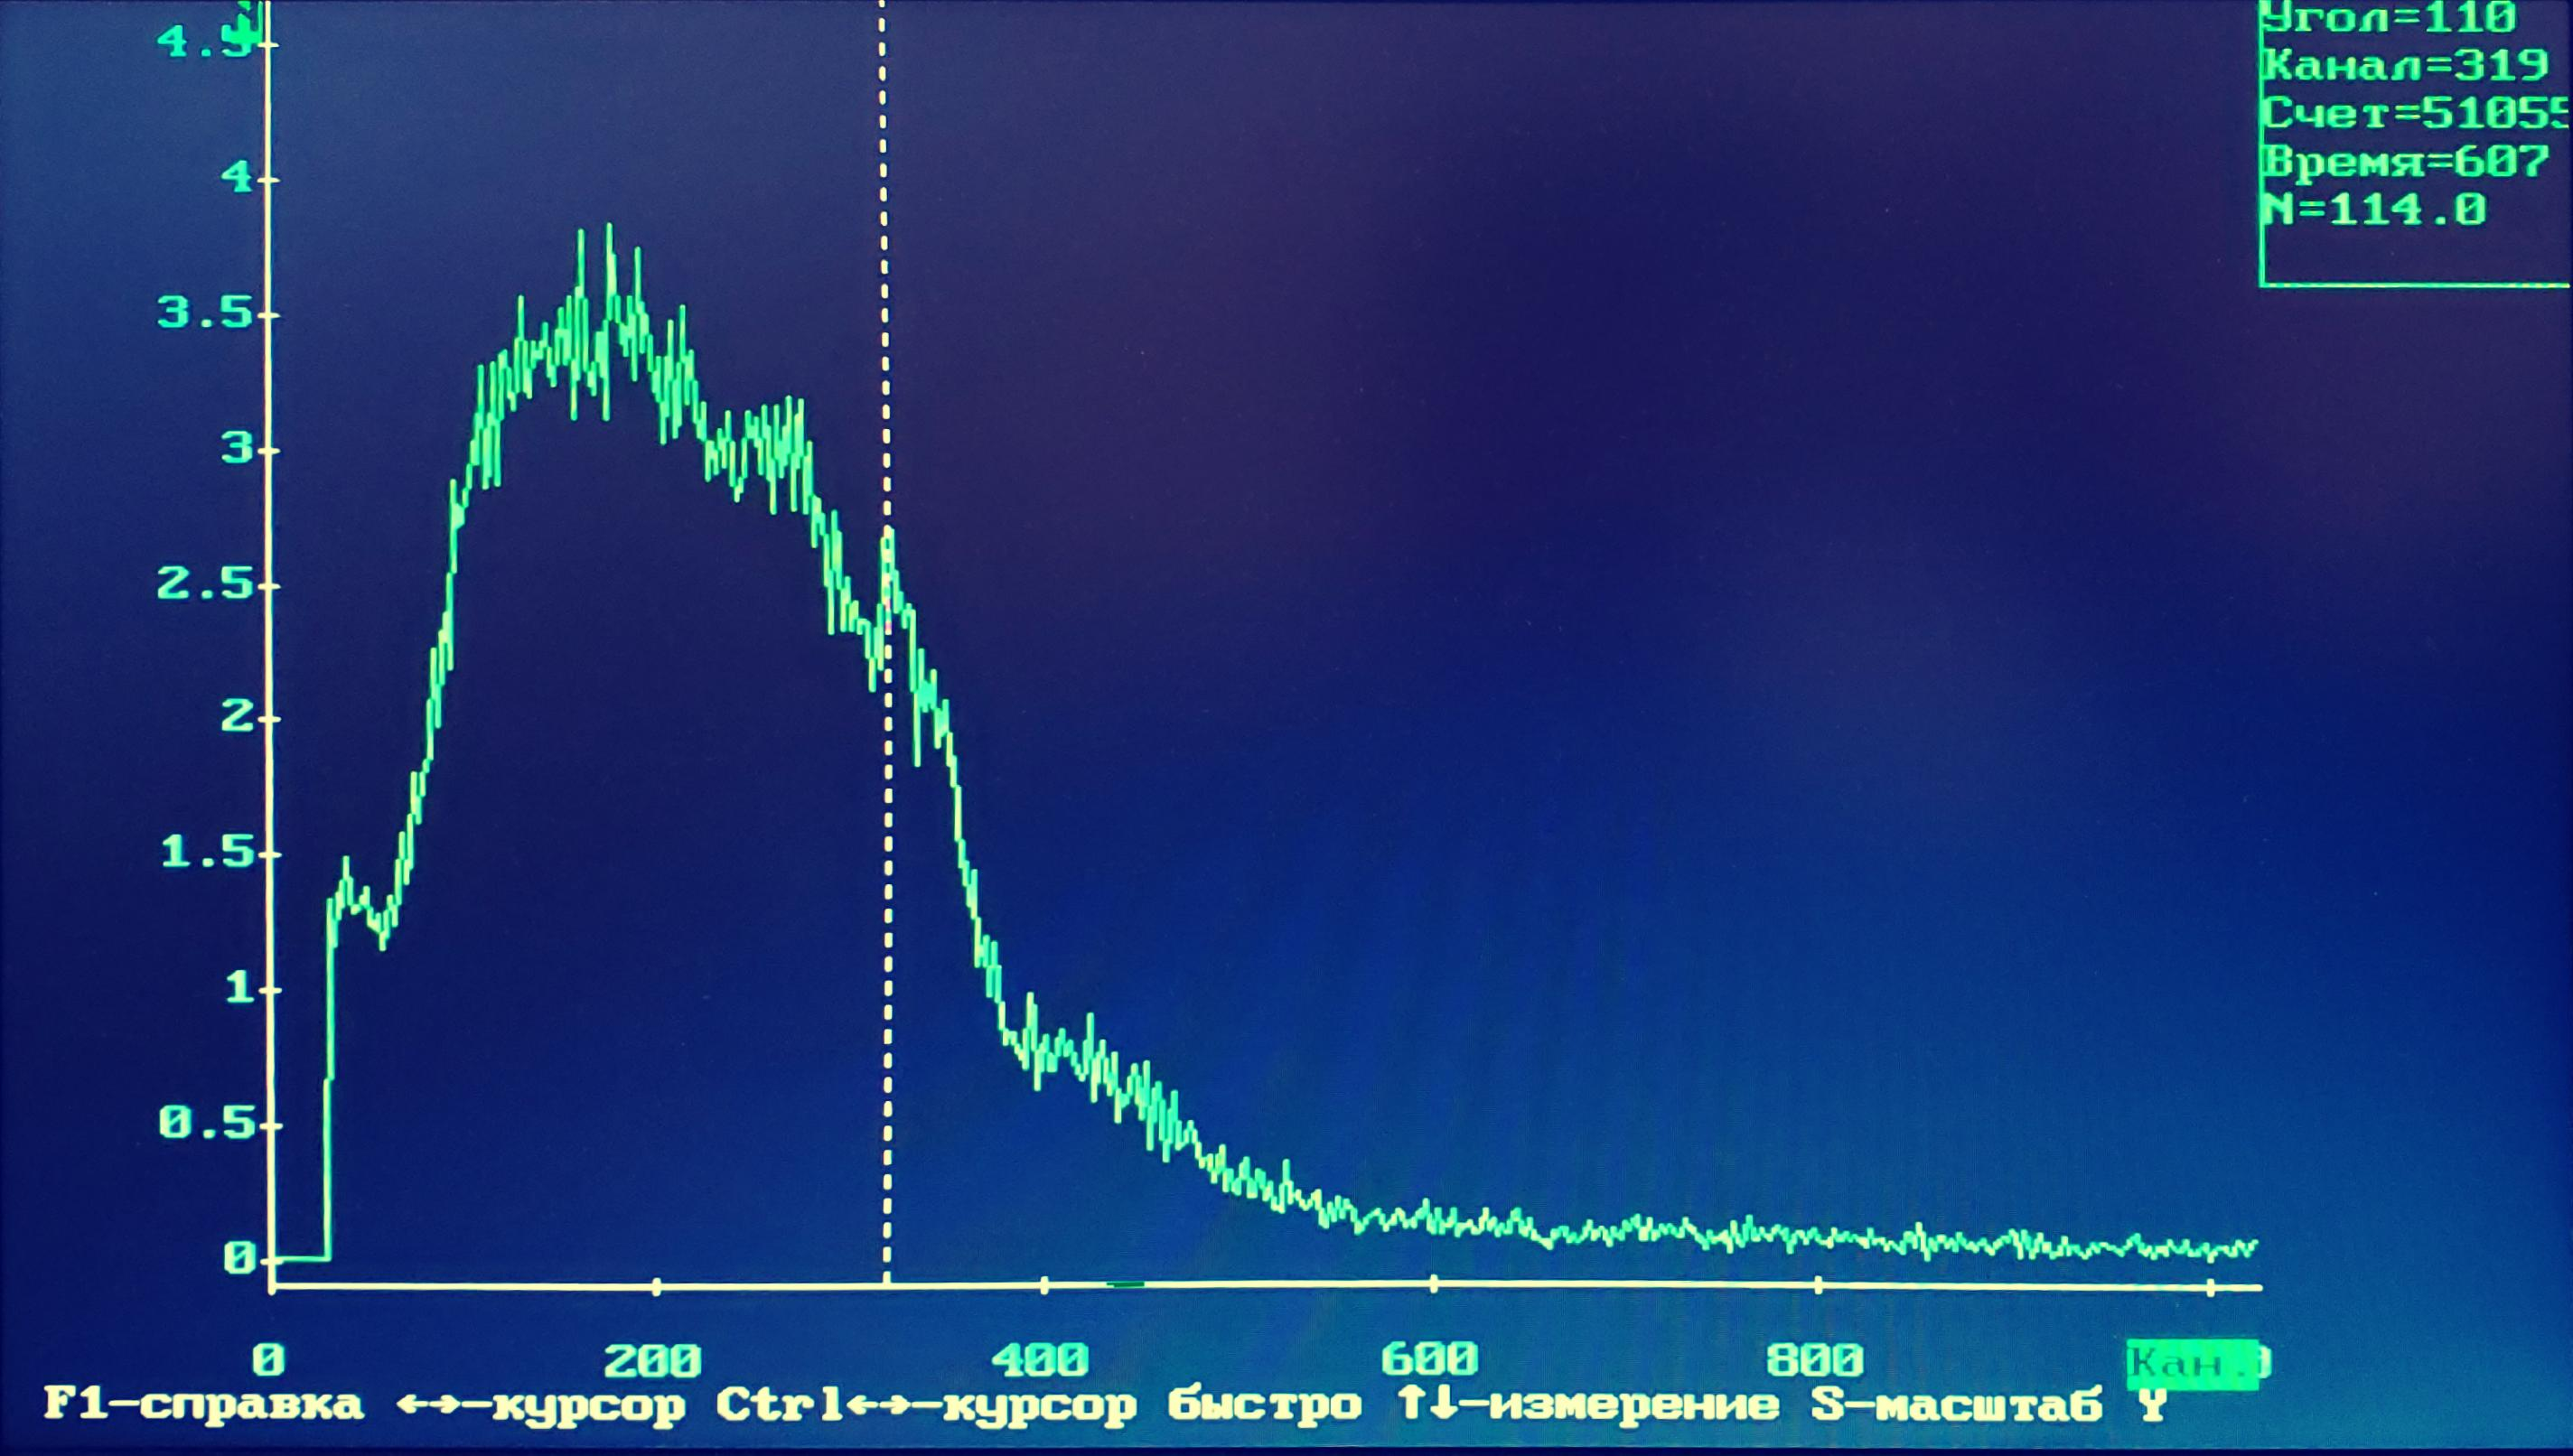
\includegraphics[width = \linewidth]{spectre110.jpg}}\\
      Рис 13. $\theta = 110^{\circ}$
    \end{minipage}
  \end{figure}
  \begin{figure}[h!]
    \begin{minipage}[h]{0.32\linewidth}
      \center{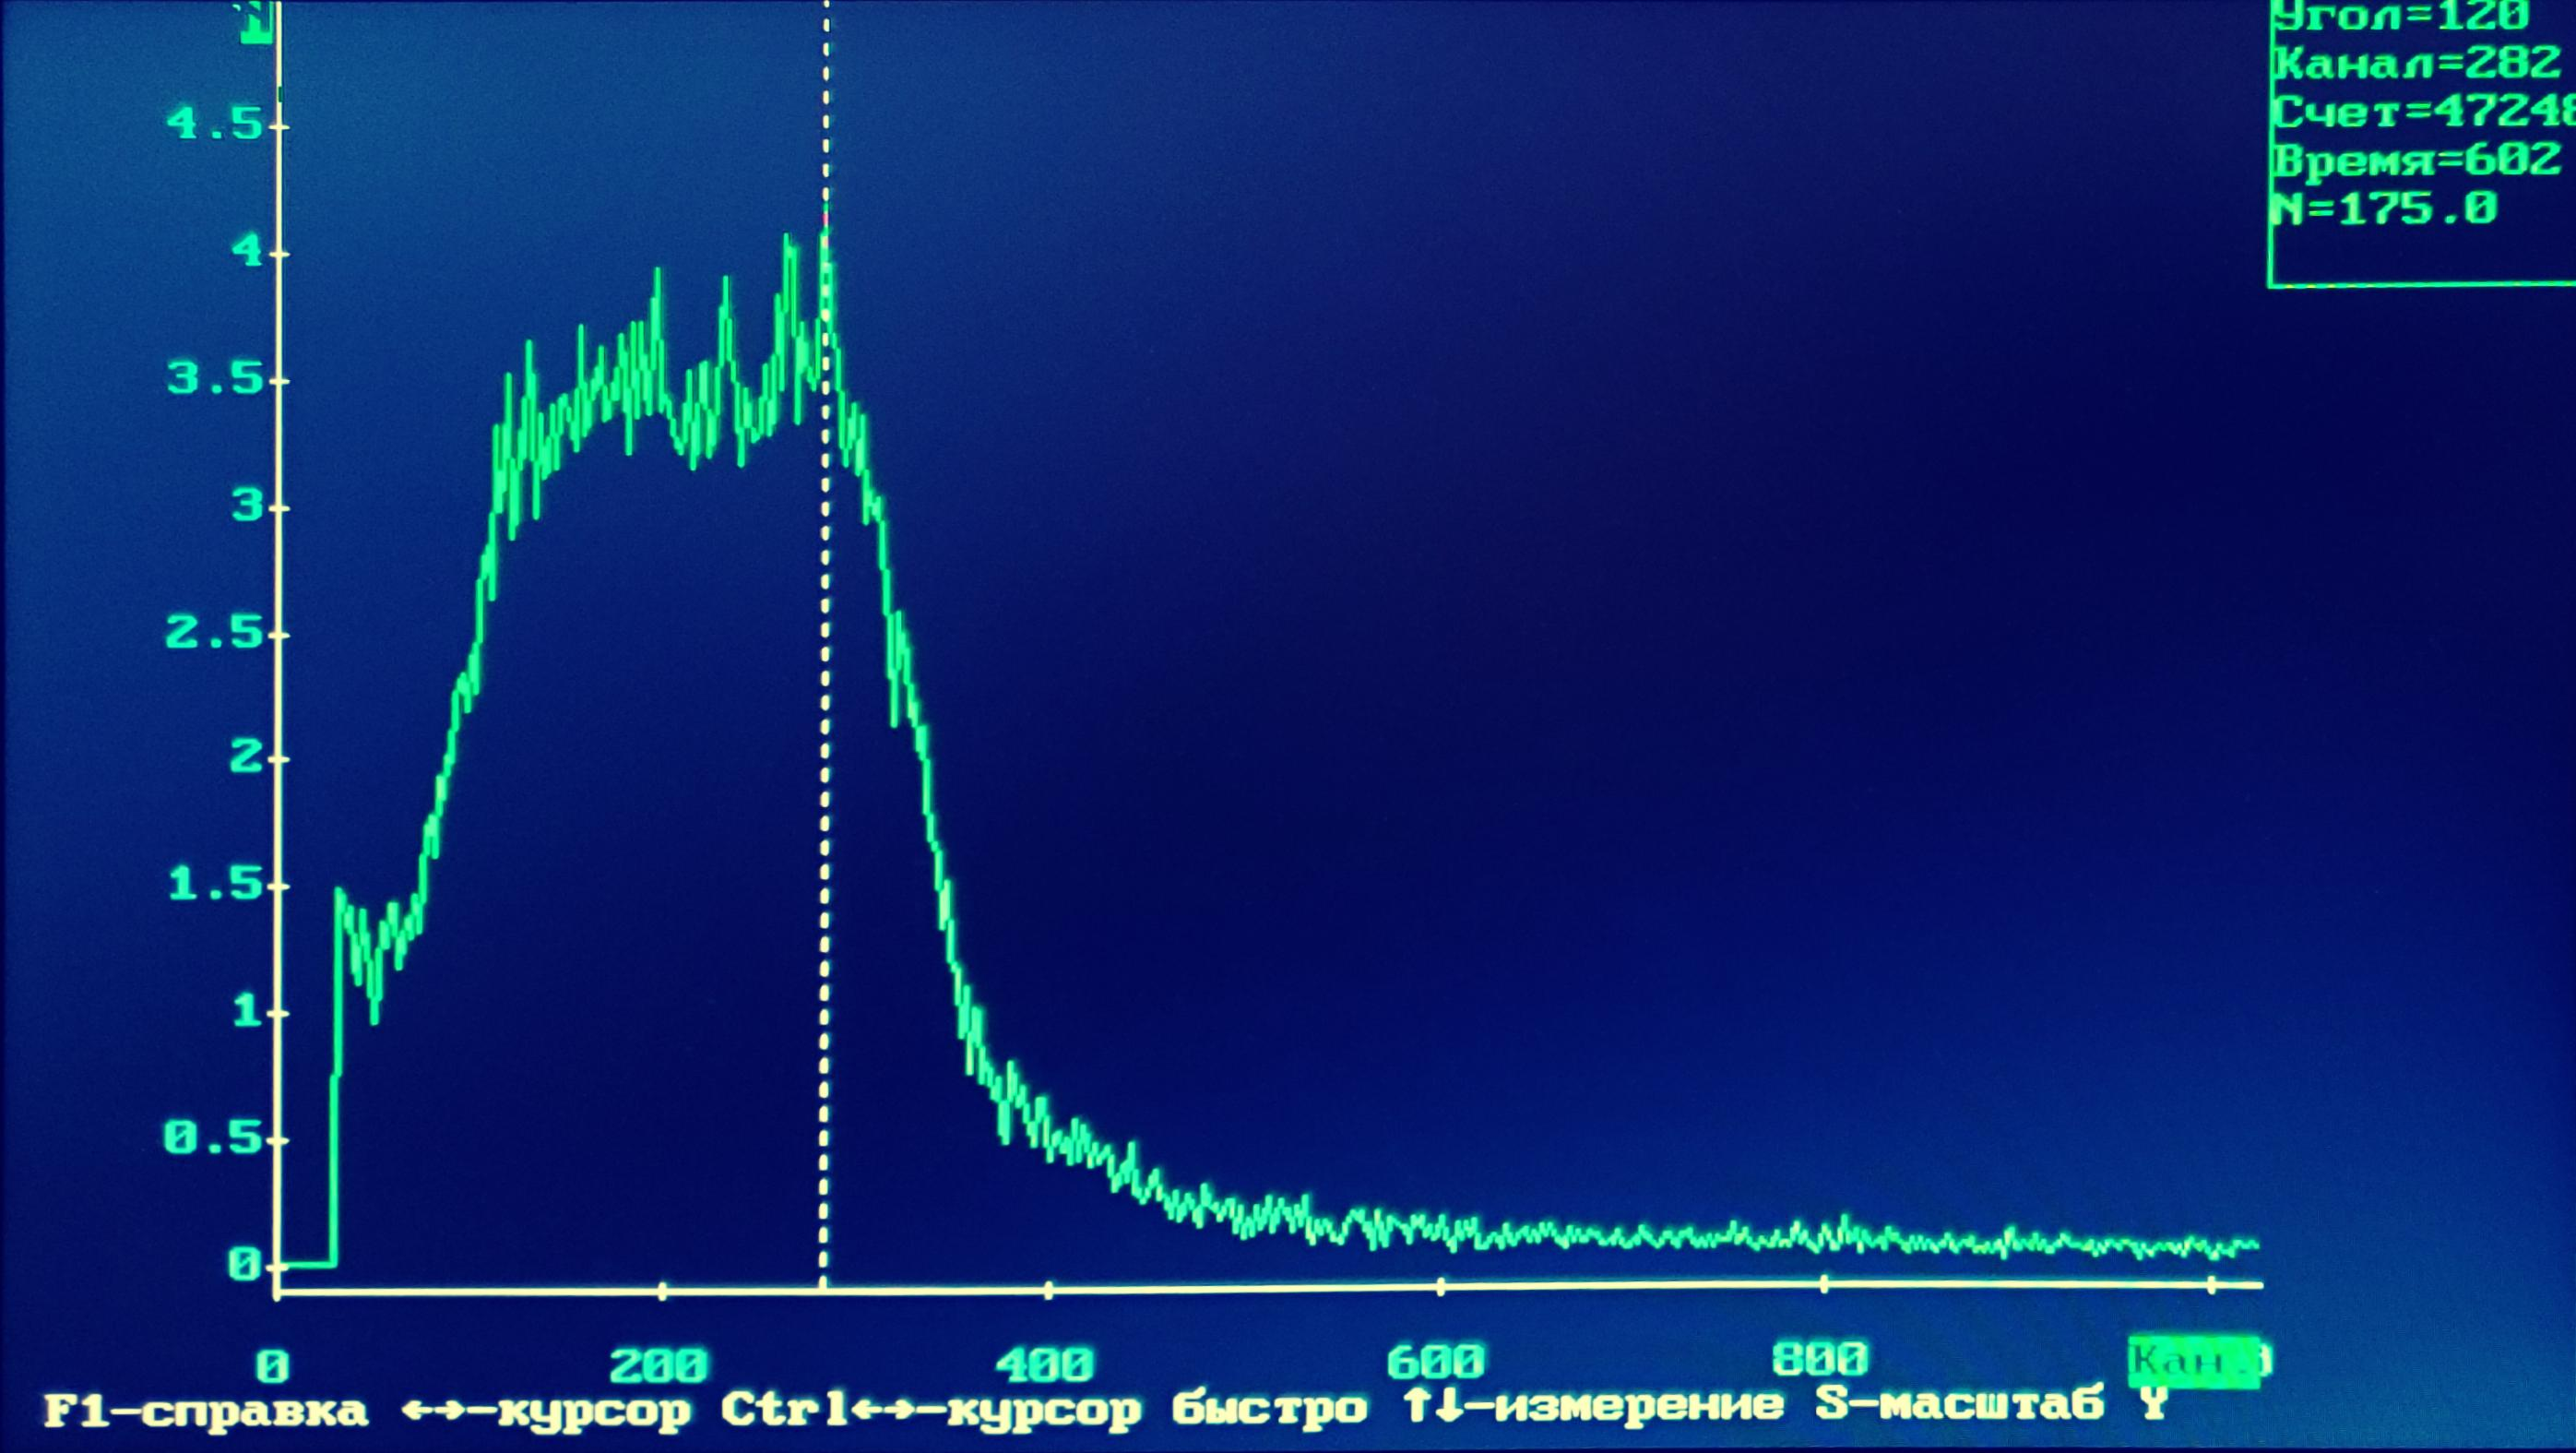
\includegraphics[width = \linewidth]{spectre120.jpg}}\\
      Рис 14. $\theta = 120^{\circ}$
      \label{fig:oscillograme}
    \end{minipage}
  \end{figure}

\end{document}
